
\documentclass[11pt]{report}

\usepackage{float}
\usepackage[utf8]{inputenc}
\usepackage{graphicx}
\usepackage{booktabs}
\usepackage{caption}
\usepackage{subcaption}
\usepackage{amsmath}
\usepackage[width=150mm,top=35mm,bottom=25mm,bindingoffset=6mm]{geometry}
\usepackage{fancyhdr}
\usepackage{setspace}
\usepackage{float}
\usepackage[table]{xcolor}
\usepackage{lscape}
\usepackage{adjustbox}
\usepackage{tabularx}
\usepackage{makecell}
\usepackage{hyperref}
\usepackage{graphicx}
\usepackage{subcaption}
\usepackage[style=numeric,sorting=none]{biblatex}
\usepackage{multirow}
\usepackage{hhline}
\usepackage[justification=centering]{caption}
\usepackage{enumitem}
\usepackage{placeins}

\pagestyle{fancyplain}
\fancyhf{}
\fancyhead[R]{\thepage}

\newcommand{\rnp}[3]{\ensuremath{\mathit{r} = #1,~\mathit{n} = #2,~\mathit{p}~#3}}

\renewcommand{\headrulewidth}{0pt}

\addbibresource{references.bib}

\graphicspath{ {images/} }

\usepackage[font=small,labelfont=bf,labelsep=period]{caption}
\captionsetup[sub]{labelfont=bf,font=small,labelformat=parens} % => (a), (b)

\setlength{\headheight}{14pt}
\setlength{\textfloatsep}{30pt plus 2pt minus 4pt} % Adjust space between floats and text
\setlength{\floatsep}{15pt plus 2pt minus 2pt}    % Adjust space between floats
\setlength{\abovecaptionskip}{10pt}                % Adjust space above caption
\setlength{\belowcaptionskip}{10pt}                % Adjust space below caption
\setlength{\parindent}{0pt}

\title{A System Of Automated Data Collection and Use Of Machine Learning To Track Flowering and Fruiting In Cranberry Plots for Berry Count Prediction }
\author{John Jewison}
\date{05 05 2025}

\begin{document}
\pagenumbering{roman} 

\begin{titlepage}
    \begin{center}
        \vspace*{1cm}
        
        \Huge
        \textbf{A System Of Automated Data Collection and Use Of Machine Learning To Track Flowering In Cranberry Plots with Yield Prediction }
        
        \vspace{0.5cm}
        \LARGE
        \vspace{0.5cm}
    
        \textbf{John Jewison}
        
        \vfill
        
        A dissertation submitted in Partial fulfillment\\
        of the requirements for the degree of\\
        Master of Science
        (Biological Systems Engineering)\\
        
    
        
        \vspace{1.8cm}

        
        \Large
        at the\\University of Wisconsin-Madison\\
        2025\\
        \vspace{1.0cm}
        \begin{flushleft}
        \large
        Date of Final Oral Exam:  08/22/2025\\
        \vspace{1.0cm}
        The dissertation is approved by the following members of the Final Oral Committee: \\
        \vspace{.5cm}
        \setlength{\parindent}{6ex}
        Dr. Matthew Digman, Associate Professor, Biological Systems Engineering\\
        Dr. Juan Zalapa,   Professor, Horticulture\\ 
        Dr. John Shutske, Professor, Biological Systems Engineering\\
        \end{flushleft}
        
    \end{center}
    
\end{titlepage}

\doublespacing

\chapter*{Dedication}

To all the dreamers, the doers, and the courageous souls stepping into uncharted territory:

This is for you—the ones who dare to leave comfort behind, to try, to stumble, to rise, and to try again. Your willingness to embrace uncertainty and explore the unknown inspires us all.

May this journey, whether smooth or rocky, ignite growth, spark joy, and remind you of the infinite strength within. Here's to every brave step you take—may it lead to a life full of discovery, resilience, and fulfillment.

Keep going. You're creating something extraordinary.

 

\chapter*{Declaration}

"I, John Jewison, hereby declare that this thesis, entitled 'A System Of Automated Data Collection and Use Of Machine Learning To Track Flowering In Cranberry Plots with Yield Prediction', is my own original work, conducted under the supervision of Dr. Matthew Digman and Dr. Juan Zalapa, and that all sources used have been duly acknowledged and referenced according to academic integrity standards. This thesis has not been submitted previously for any other degree, and all materials included are my own unless otherwise cited."

  \vspace{0.5cm}
\begin{tabular}{@{}p{.5in}p{4in}@{}}
Signed: & \hrulefill \\
& John Jewison \\
\end{tabular}

\chapter*{Acknowledgments}

I want to thank all those that have supported and helped me through my studies at the University of Wisconsin-Madison. As a non-traditional graduate student, the learning environment can feel challenging, and relating to other students can seem more difficult. However, it was easier to overcome these feelings by reaching out to those around me, both personally and within the academic environment at UW.

To Dr. Juan Zalapa, who I am indebted to for not just teaching me as much as he could about cranberries but for sharing his infectious enthusiasm and passion for the berries. For guiding me to the answers I needed and to the questions that I should ask. 

My sincere gratitude to Dr. Matthew Digman, who first persuaded me to continue my pursuit of education after leaving the academic world, and for making it easier to transition back with his advice and guidance.  

A special thank you to all the fellow students who helped me on this project, whether collecting data or simply sharing good times together; they truly did make the load feel lighter and the task feel less impossible.

This research was possible thanks to the financial support of the Cranberry Growers Board as well as knowledge shared by individual  growers, in addition to the assistance of  the staff at the Wisconsin Cranberry Research Station.

Finally, I am immensely thankful to my new wife Natalie for her loving support and encouragement as we take on yet another ambition.

\newpage

\fancyhf{} % clear all header and footer fields
\fancyhead[RO,R]{\thepage} %RO=right odd, RE=right even
\renewcommand{\headrulewidth}{0pt}

\begin{center}
    
    \vspace{0.9cm}
    \textbf{Abstract}
\end{center}

\doublespacing

The American cranberry (\textit{Vaccinium macrocarpon} Ait.) is a high-value specialty crop, with Wisconsin producing over 60\% of the U.S. harvest \cite{usda-nass_cranberries_2024}. Due to this importance, accurate and early yield prediction is critical for efficient crop management and harvest planning, yet existing approaches are labor-intensive, inconsistent, and often restricted to low-frequency manual scouting \cite{haufler_microwave_2022}. Recent advances in machine learning and agricultural robotics offer new opportunities to overcome these limitations \cite{ni_deep_2020,cinat_comparison_2019}.

This study presents an automated ground-based robotic imaging platform paired with deep learning models to track flowering and fruit set across 626 cranberry breeding plots over twelve imaging sessions. A custom dataset was created using the Segment Anything Model for image annotation \cite{kirillov_segment_2023}, enabling training and evaluation of object detection architectures including YOLOv11 \cite{jocher_ultralytics_2023}, YOLOv12, and RF-DETR \cite{robinson_rf-detr_2025}. Model performance was evaluated using precision, recall, and F1-score metrics. The YOLOv12 model achieved a mean precision of 0.79, recall of 0.66, and an F1-score of 0.72 across validation sets, while RF-DETR produced more accurate results (precision = 0.77, recall = 0.70, F1 = 0.73). Inference speeds were also benchmarked to support real-time and in-field deployment.

Flower counts predicted by the best-performing models were correlated with ground-truth berry counts at harvest. Statistical analysis demonstrated significant positive correlations ($r = 0.68$, $p < 0.001$) between flower density and final berry yield, confirming that flowering intensity is a reliable predictor of fruit set. Regression models showed that both the timing and concentration of flowering events contributed to variation in berry production, highlighting the importance of repeated sampling throughout the flowering season \cite{brown_fruit_2006,parent_current_2021}.

By integrating robotics with image-based deep learning, this system reduces sampling time, improves data resolution, and enables year-round monitoring. The approach provides a scalable framework for cranberry breeding, yield forecasting, and precision management, and can be extended to other specialty crops facing similar challenges in high-resolution monitoring \cite{loarca_berryportraits_2024}.


\tableofcontents

\listoffigures

\listoftables

\pagenumbering{arabic} 

\chapter*{General Introduction}
Cranberries (\textit{Vaccinium macrocarpon}) are a unique and valuable fruit native to North America, widely recognized for their distinctive tart flavor, vivid red color, and nutritional benefits. Rich in antioxidants, vitamins, and dietary fiber \cite{blumberg_impact_2016}, cranberries have long been celebrated for their potential health benefits such as supporting cardiovascular function and providing anti-inflammatory properties \cite {leahy_cranberry-promising_2001}. Due to these benefits, a surge in consumer demand for cranberry-based products, ranging from fresh berries and juices to supplements and extracts. To help fill this demand, cranberry producers have shown an increasing interest in the incorporation of new technology in multiple areas of production \cite{jackson_case_2021}, from crop maintenance and pest control to harvest and processing \cite{johnson_ml_cranberry_2008}. 

While mechanization and precision farming techniques have become ubiquitous, particularly in grain and row-crop farming \cite{hameed_technology_2025}. Large-scale use is easier to implement and costs are spread onto thousands of acres and integrated into fewer and larger machines used across all those acres. However, the use of such technology has been slower in crops used for food production, such as vegetables and berry production, because crop and field sizes are generally smaller and economies of scale are more difficult to realize.

Fortunately, as technology has evolved in recent decades, consumer use has pushed robotics and mechatronics into smaller and smaller form factors and, importantly, used this widespread use to reduce production and implementation costs. Power storage in the form of new generations of batteries paired with economical forms of generation such as solar has given robotics the ability to perform more power-intensive jobs, or the ability to do those jobs over extended durations.  On the other side of the power equation, more compact and powerful motors and actuators have been able to more efficiently use this energy provided to accomplish a wide variety of tasks from crop harvesting \cite{das_designing_2024} to weeding and seeding operations \cite{vahdanjoo_operational_2023}

Alongside consumer use and demand for smaller, more powerful mechatronics, hobbyist development of electronic control for systems ranging from drones to 3D printing has made the level of entry into precision computerized control of mechatronics systems a smaller hurdle when developing small-scale systems. No longer are large multi-disciplined teams of software and electronics engineers needed, but systems can be built up from preassembled parts of open-sourced software with wider support from internet-based communities.

Although machine learning has been used in other fruiting crops for both fruit and flower detection, it is generally done at one time during flowering \cite{lee_detection_2021} to estimate the fruit count or is used after fruit development to help predict crop ripeness \cite{villacres_detection_2020}. This study aims to improve on those works by increasing the sampling rate to multiple times during the flowering to allow for tracking both flower count and duration as well as including a connection between flowering and fruit set by collecting data both during and after flowering to record fruit set and early fruit development. In order to produce consistent data in a controlled way, automation is used to both decrease sampling intervals and reduce variables such as image timing, image resolution, orientation, and ground sampling distance. This will be accomplished by using a purpose-built automated ground vehicle (AGV) that is able to traverse the cranberry bog autonomously.  This AGV will be able to sample and track images and store the data.



\addcontentsline{toc}{section}{General Introduction}

\chapter*{Thesis Objective}
This thesis aims to provide an example of the use of automation, crop imaging, and machine learning as a system to better understand and predict plant flowering and fruit set. Flowering is a crucial phase in the cranberry growth cycle, as it directly influences berry formation, yield, and overall crop quality. Understanding the complex dynamics of cranberry flowering, including factors such as floral initiation, development, and pollination, is essential to optimize cultivation practices and improve productivity.  This process is influenced by a range of factors, including the environment and genetics. Plant nutrients, precipitation levels, and temperature also represent external factors that affect the timing and success of flowering.

Specifically, we will build and document an autonomous imaging platform and survey workflow that will train and compare modern detectors (YOLOv11/YOLOv12/RF-DETR/RF3) on a labeled dataset ($\geq$1,400 images; $\geq$50k instances) for flower/early-fruit detection. After training, we will select a deployment-feasible model meeting mAP@0.50 $\geq$ 68\% and single-image latency $\leq$ 75~ms at $640 \times 640$, and finally test the association between total flower count (aggregated over a standardized bloom window) and total berry count using OLS and cross-validated predictive error, with pre-specified subgroup analyses by cultivar (Stevens vs. Experimental hybrids).

As a result of this study, better methods for analyzing and tracking the timing and extent of cranberry flowering will offer producers the ability to make more informed and timely decisions about crop management. In addition to crop production, an improved yield estimate will allow for more efficient downstream supply chain planning and marketing. Furthermore, this project will aim to demonstrate the potential use and future expansion of autonomous ground vehicles to collect and process image data, as well as to incorporate additional sensors to further improve crop management and yield prediction.

\addcontentsline{toc}{section}{Thesis Objective}

\chapter{An Automated Data Collection Platform}
\section{Abstract}

\begin{singlespace}
Cranberries (\textit{Vaccinium macrocarpon}) are a high-value specialty crop, with the United States producing nearly 97\% of the global supply and Wisconsin contributing over 60\% of the domestic harvest \cite{usda-nass_cranberries_2024}. Monitoring cranberry growth and yield is particularly challenging because of the crop’s unique cultivation in sandy, low-lying marshes, the low stature of cranberry vines, and the small size of blossoms and fruit. Current monitoring approaches rely heavily on manual data collection or aerial imagery, which can be labor-intensive, inconsistent, or resolution-limited. This study presents the design and testing of a low-cost, ground-based robotic imaging platform tailored for cranberry research and smaller producers. The rover was designed to navigate sandy soils and narrow aisles in genetic phenotyping cranberry beds, collecting high-resolution RGB imagery of blossoms and fruit while minimizing disturbance to the crop. Field testing demonstrated the system’s robustness under variable conditions, capturing imagery suitable for bloom density assessment, yield estimation, and future machine learning applications. By offering an open-source, low-maintenance design that integrates autonomous navigation and precision imaging, this platform has the potential to expand access to advanced monitoring tools, reduce labor costs, and support data-driven management decisions in cranberry production.
\end{singlespace}

\newpage

\section{Introduction}

The integration of robotic imaging technology into agriculture is transforming how crops are monitored and managed by providing precise, real-time data on plant health, growth stages, and yield estimation \cite{cinat_comparison_2019}. Ground-based robotic rovers equipped with RGB, multispectral, and hyperspectral cameras can collect high-resolution imagery under consistent conditions, overcoming many of the altitude and lighting limitations of aerial platforms \cite{wendel_self-supervised_2016}. When combined with computer vision and machine learning algorithms, these systems have shown promise for detecting plant stress \cite{abebe_image-based_2023}, quantifying flowering, and improving yield predictions with greater accuracy than traditional sampling methods.

While these advances are well documented in crops such as tomatoes \cite{seo_development_2021}, lettuce \cite{hu_lettucetrack_2022}, and peppers \cite{lehnert_autonomous_2017}, specialty crops like cranberries present unique challenges. Cranberries are grown in sandy, acidic marshes across northern U.S. states, with Wisconsin and Massachusetts accounting for the majority of production \cite{usda-nass_cranberries_2024}. Unlike orchard or row crops, cranberries form low, vine-like mats with blossoms and fruit borne close to the ground \cite{sandler_cranberry_2008}. Monitoring bloom density and berry set is labor-intensive and prone to sampling error, yet these factors directly influence pollination success and yield. Furthermore, cranberry production faces persistent threats from fungal fruit rot complexes and insect pests, where timely detection and intervention are critical \cite{oudemans_cranberry_1998}.

Despite advances in robotics for other crops, cranberry monitoring remains reliant on on manual field scouting or aerial imagery, both of which present limitations. Manual scouting is time-consuming and constrained in spatial coverage, while aerial imagery often lacks the resolution necessary to detect individual cranberry flowers or small fruits. These unique agronomic and environmental conditions create an opportunity for lightweight, ground-based robotic rovers that can provide consistent, high-resolution data without damaging the crop.

This study presents the development and field validation of a purpose-built robotic rover designed to meet these challenges. The platform integrates high-resolution imaging, autonomous navigation, and robust frame design into a compact system optimized for cranberry marsh conditions. By addressing the barriers of cost, usability, and crop-specific constraints, the system aims to expand access to precision agriculture technologies for small and mid-sized cranberry producers, enabling more efficient bloom monitoring, improved yield estimation, and enhanced long-term crop management.


\section{Design}

The UGV was designed to traverse the grid system of test plots using the separation aisles between plots in order to minimize disturbance to the plants. Navigating the marsh proved to be a challenging task while providing a stable imaging platform. Any unnecessary disturbance needed to be avoided as it would potentially affect flower pollination. To improve overall mobility, a wheeled skid-steering type rover was chosen. This choice allowed the use of large diameter wheels necessary to navigate the sandy soil type while still allowing the rover to perform pivot-style turns at the end of each grid column.

\subsection{Frame}
The rover was modeled in Creo Parametric \cite{ptc_creo_2023} with multiple revisions considered. To allow for easier modification, the frame was designed with primarily bolted connections. This allows for modification of dimensions as well as changing out entire sections of the robot. An isometric view of the model can be seen in Figure~\ref{fig:Initial CAD Model}. Steel was chosen for the primary frame material due to its low relative cost and ease of manufacture. Aluminum was used for auxiliary brackets and supports including the camera mount. Although the steel structure resulted in an increased weight compared to an aluminum frame, the total weight of the frame excluding wheels and electronics was relatively low at 72 lbs. Considering the entire weight of the robot of 138 lbs, the frame only accounts for less than 60\% of the total weight.


\begin{figure}[!ht]
    \centering
    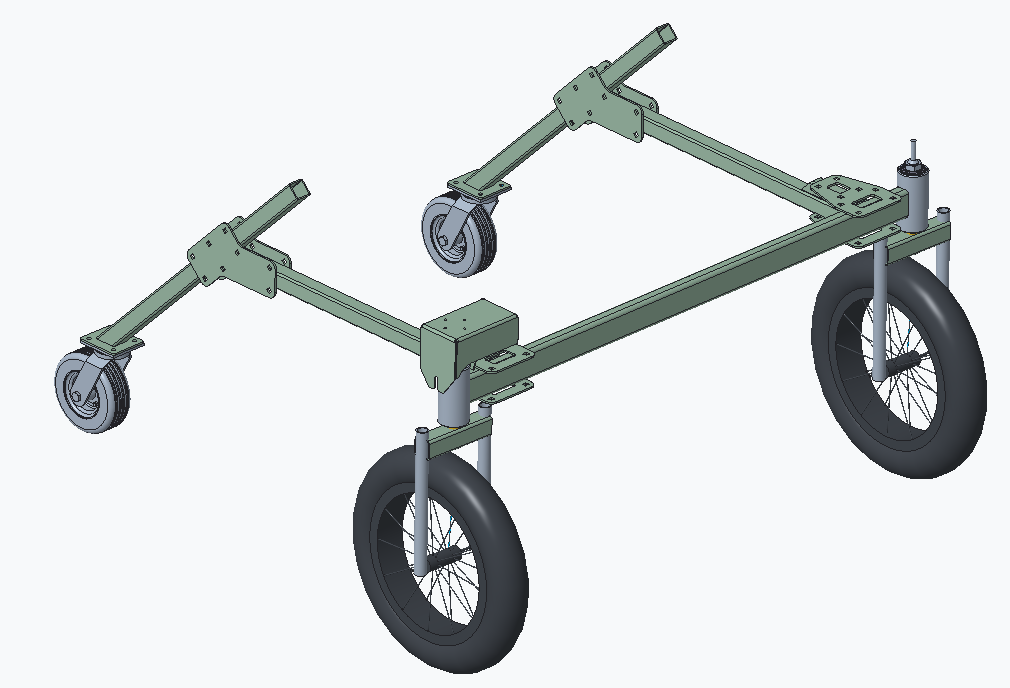
\includegraphics[width=0.75\linewidth]{images/CAD.png}
    \caption{Autonomous rover—3D CAD overview. The isometric view shows the two-wheel differential-drive layout with steerable front wheels. Note all joints between the front drive wheels and rear caster wheels are accomplished with bolted plates}

    \label{fig:Initial CAD Model}
\end{figure}

Control and steering were considered as likely systems to need to be tested and modified, so two systems were implemented in the initial design. The primary system was a differential steering system; this style  was chosen as it would provide simple control as well as good maneuverability. The secondary system was a pivoting wheel system where the main drive wheel could be rotated relative to the vehicle frame as seen in Figure~\ref{fig:steer}. This system would allow the main wheels to be pivoted around their vertical axis independently, controlled by a stepper motor (23HS22-5004D-E1000, STEPPERONLINE, China) attached to a NEMA 23 10:1 worm drive gearbox (Generic, China). A stepper motor was chosen for its low power consumption, and when coupled with a worm drive gearbox, this would allow the robot to maintain the steering position with no additional power due to the worm drive gearbox's self-locking characteristics.

\begin{figure}
    \centering
    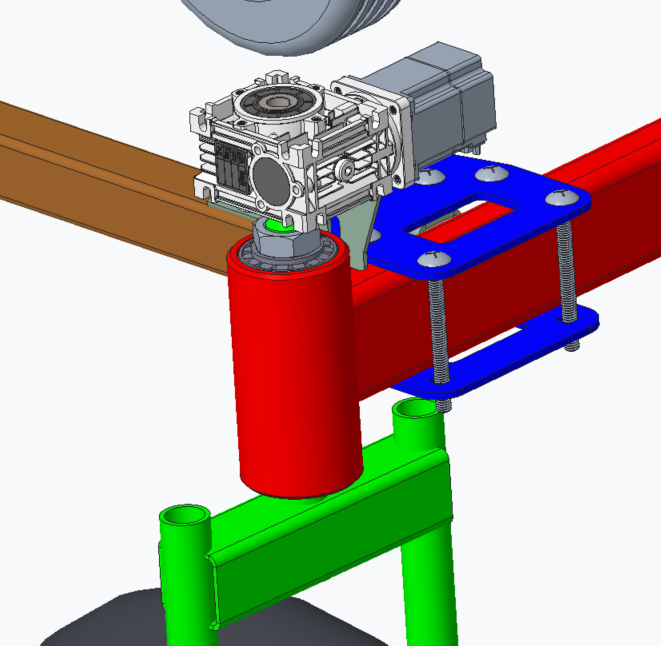
\includegraphics[width=0.75\linewidth]{images/secondary steering.png}
    \caption{Steering motor and gearbox assembly. A NEMA-23 stepper coupled to a 10:1 worm gearbox provides self-locking hold torque, allowing precise steering without continuous power draw. The assembly mounts above the drive axis for easy servicing and keeps moving parts clear of vegetation.}

    \label{fig:steer}
\end{figure}

\subsection{Sensing platform}

Two imaging systems were investigated, the first being a RealSense D435i (Intel, USA) and the second being a Canon PowerShot A810a (Canon U.S.A, USA). The Canon digital camera was selected due to better performance in most lighting conditions as well as a significantly higher image resolution. The camera was able to be interfaced with the UGV controller. The Canon captured a 16MP RGB image of size 4608 px $\times$ 3456 px and a maximum field of view of 65 degrees.  Images were captured at a height of 1500 mm and with the field of view controlled such that an area approximately 1200 mm $\times$ 1700 mm was captured. This FOV and image resolution gave a ground sampling distance (GSD) of approximately 0.37 mm/px. This resolution was chosen as a typical blossom was found to be approximately 6.3 mm to 9.5 mm \cite{diaz-garcia_image-based_2018}, with some features such as individual petals being smaller. The combination of flower size and GSD ensured approximately 15-20 pixels per flower. Images were captured using natural lighting in early afternoon to provide minimal self-shadowing and to avoid shadowing from the image collection platform.


The consideration of image lighting was a major concern to ensure that the images were as uniform as possible before any analysis was performed. The images were collected in full and partial sun as well as under a canopy that blocked all direct and ambient sunlight and used controlled artificial lighting. The best results were found using natural lighting with a solar elevation angle roughly equal to the field of view of the camera system.
    
\begin{figure}[!ht]
  \begin{subfigure}{0.3\textwidth}
    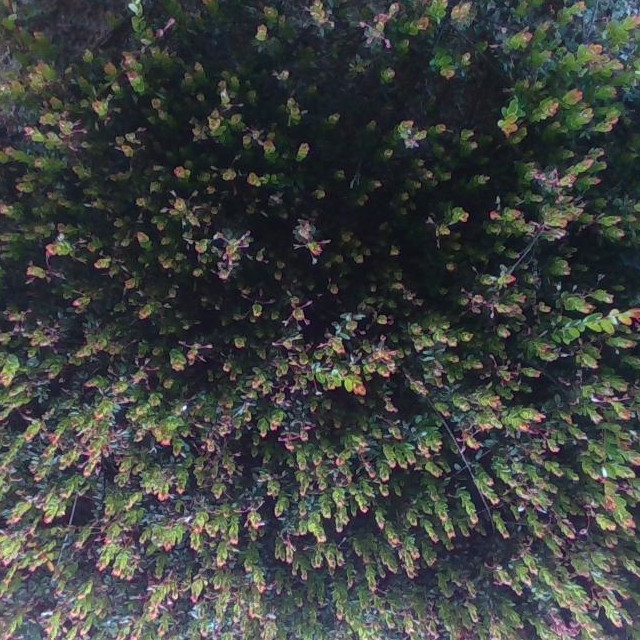
\includegraphics[width=\textwidth]{images/No-Light_7-119.JPG}
   \caption{Shaded Image}
    \label{fig:NoLight}
  \end{subfigure}
  \hfill
  \begin{subfigure}{0.3\textwidth}
    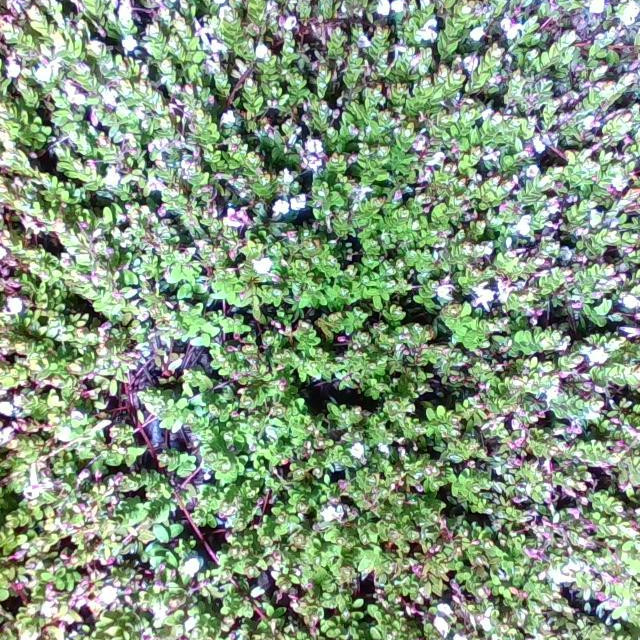
\includegraphics[width=\textwidth]{images/Artficial-Light_7-119.JPG}
   \caption{Artificial Lighting}
    \label{fig:ArtficialLight}
  \end{subfigure}
  \hfill
  \begin{subfigure}[b]{0.3\textwidth}
    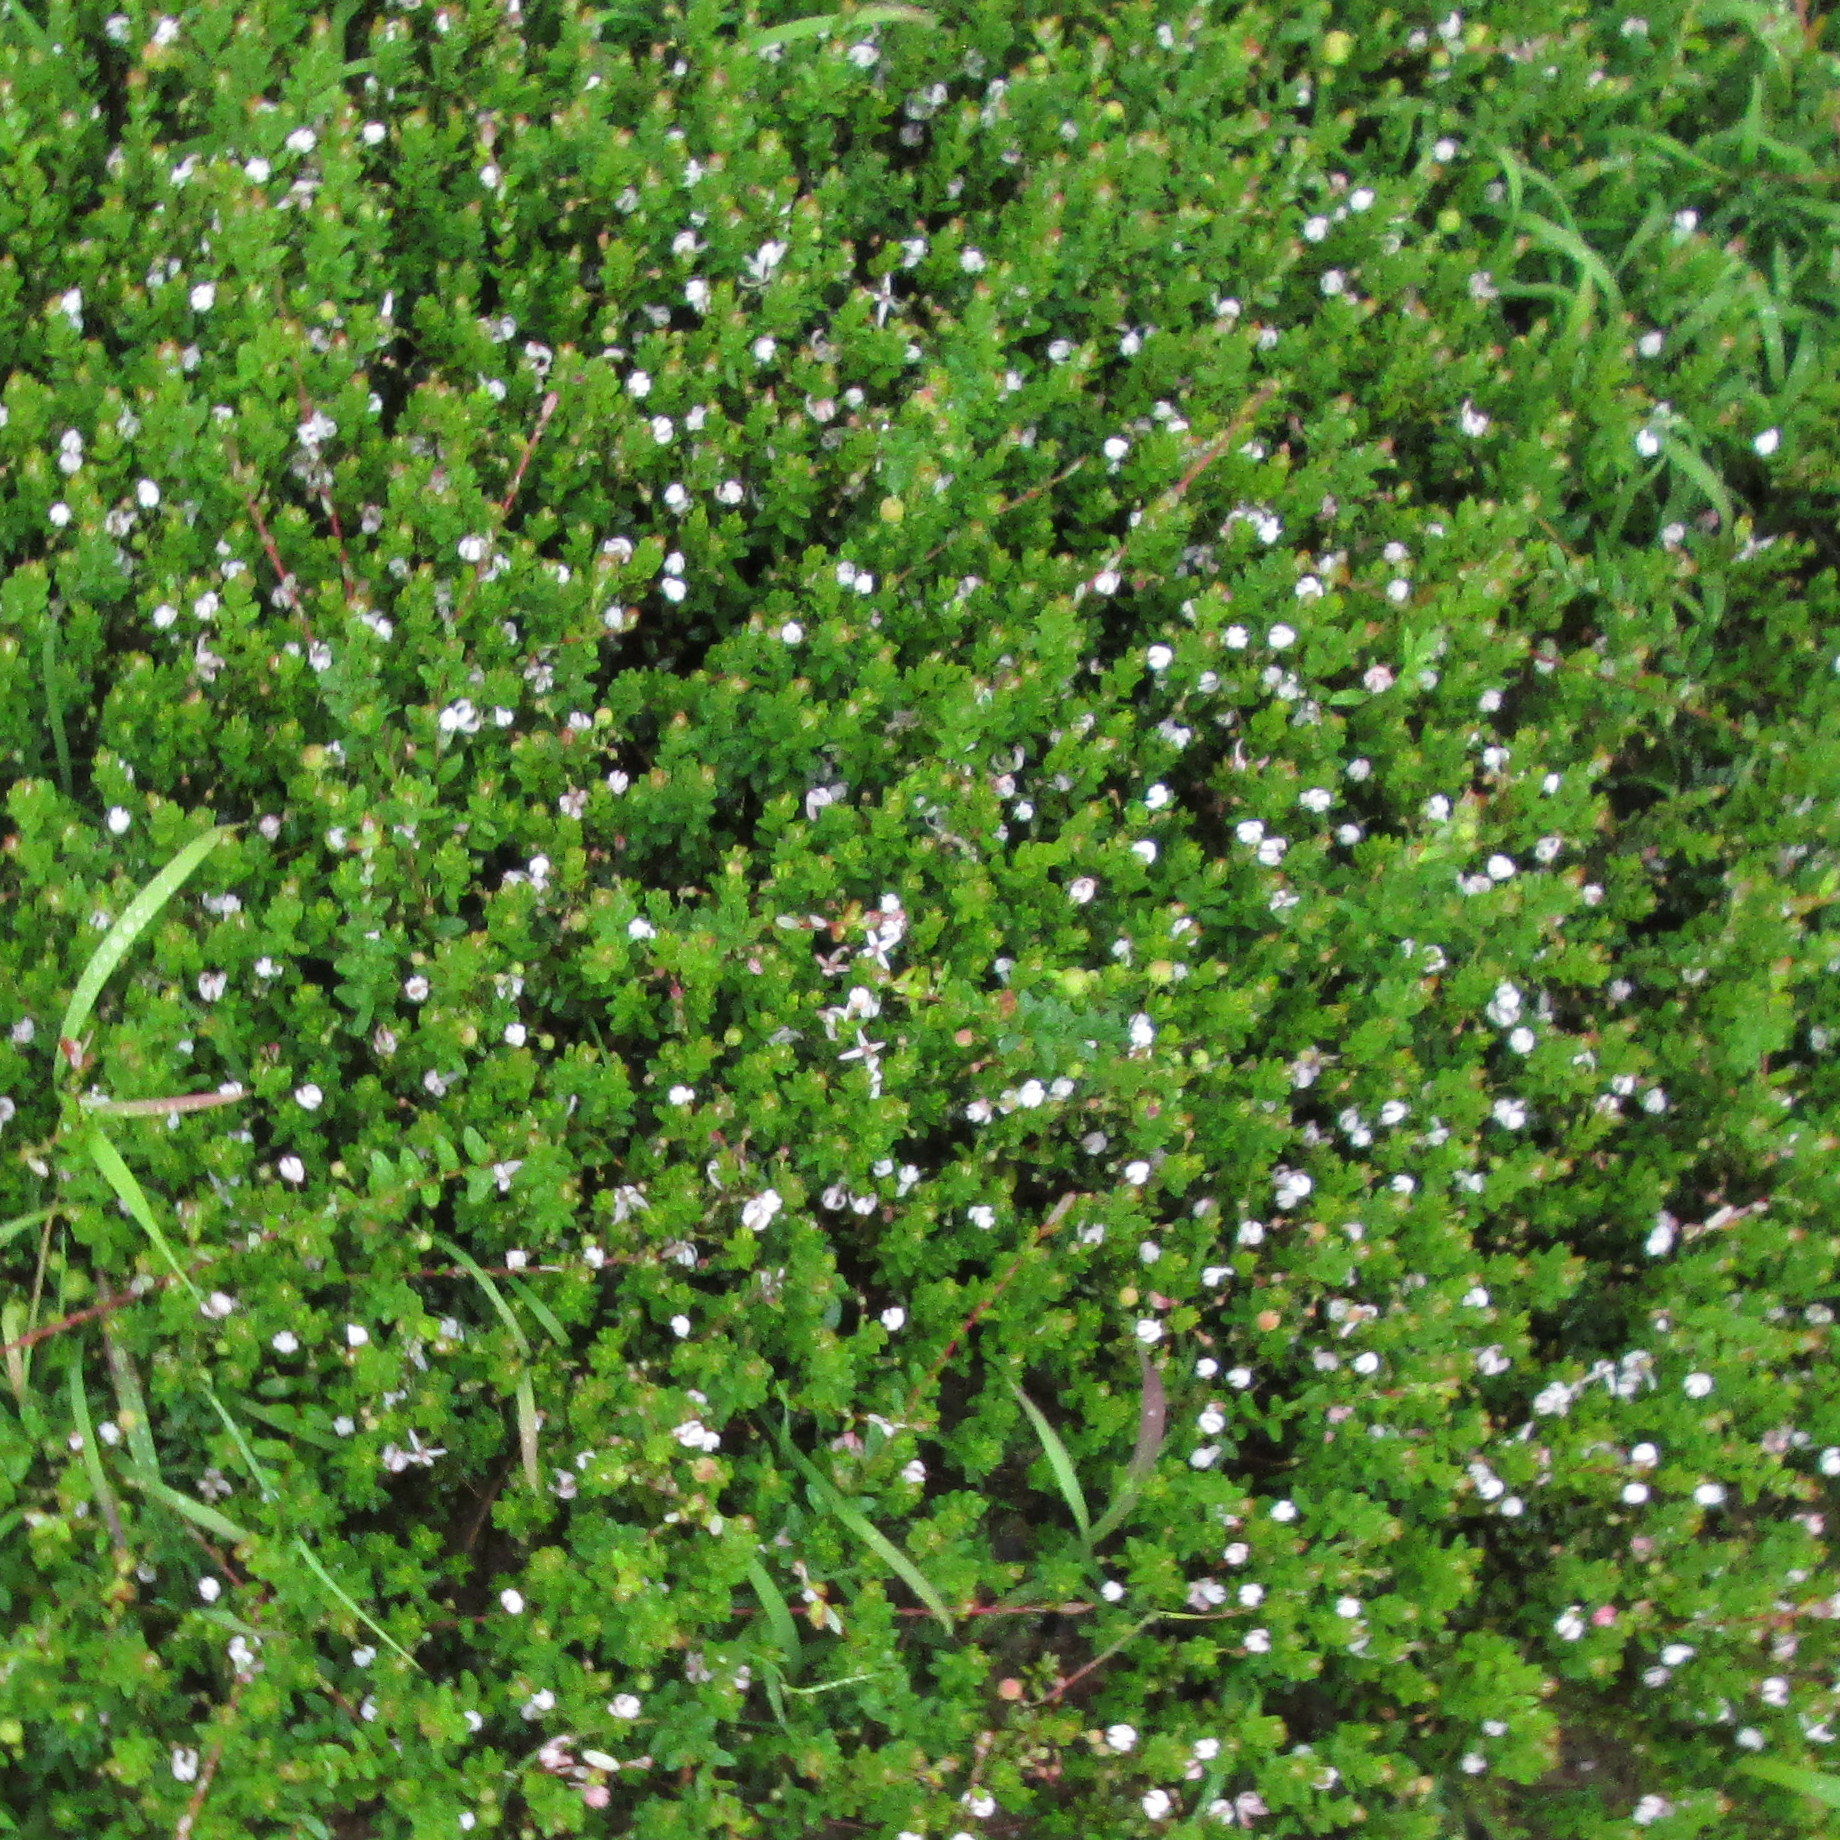
\includegraphics[width=\textwidth]{images/Nat_light_7-119.JPG}
    \caption{Natural Lighting}
    \label{fig:NaturalLight}
  \end{subfigure}
  \caption{Lighting conditions evaluated for image collection. (a) Shaded imaging reduces highlights but lowers contrast on floral structures. (b) Artificial lighting under a canopy yields stable exposure but introduces color cast and specular artifacts on glossy leaves. (c) Natural sunlight with mid-day solar elevation gave the most consistent separation of petals and foliage at our working height, so it was adopted for the main survey.}

  \label{fig:LightComp}
\end{figure}
    
In an effort to further minimize shadowing, the camera was mounted remotely to the A-UGV on an elevated arm in front of the primary structure, as shown in Figure~\ref{fig:CamMount}. The path of the A-UGV could also be optimized to avoid producing interfering shadows; typically, this was realized by traveling in a North-South direction, thus shadows produced were to the left or right of the plot being imaged.

\begin{figure}[!ht]
  \begin{subfigure}{0.4\textwidth}
    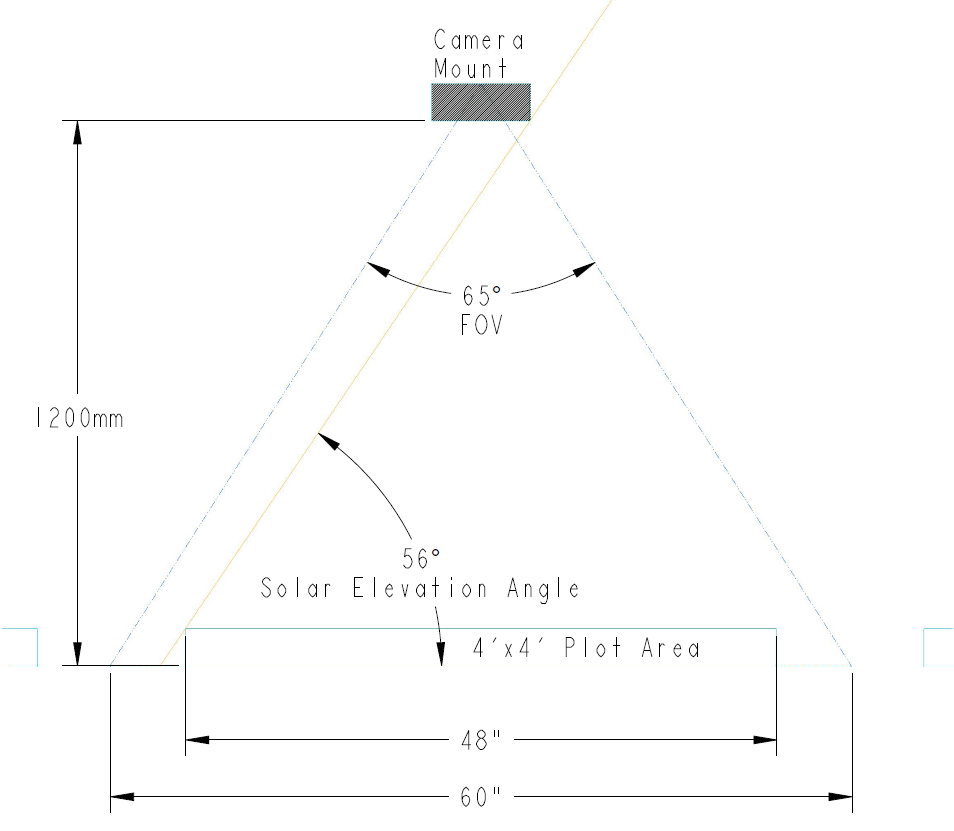
\includegraphics[width=\textwidth]{images/Sun Angle.png}
   \caption{Solar elevation relative to camera}
    \label{fig:SolAng}
  \end{subfigure}
  \hfill
  \begin{subfigure}[b]{0.4\textwidth}
    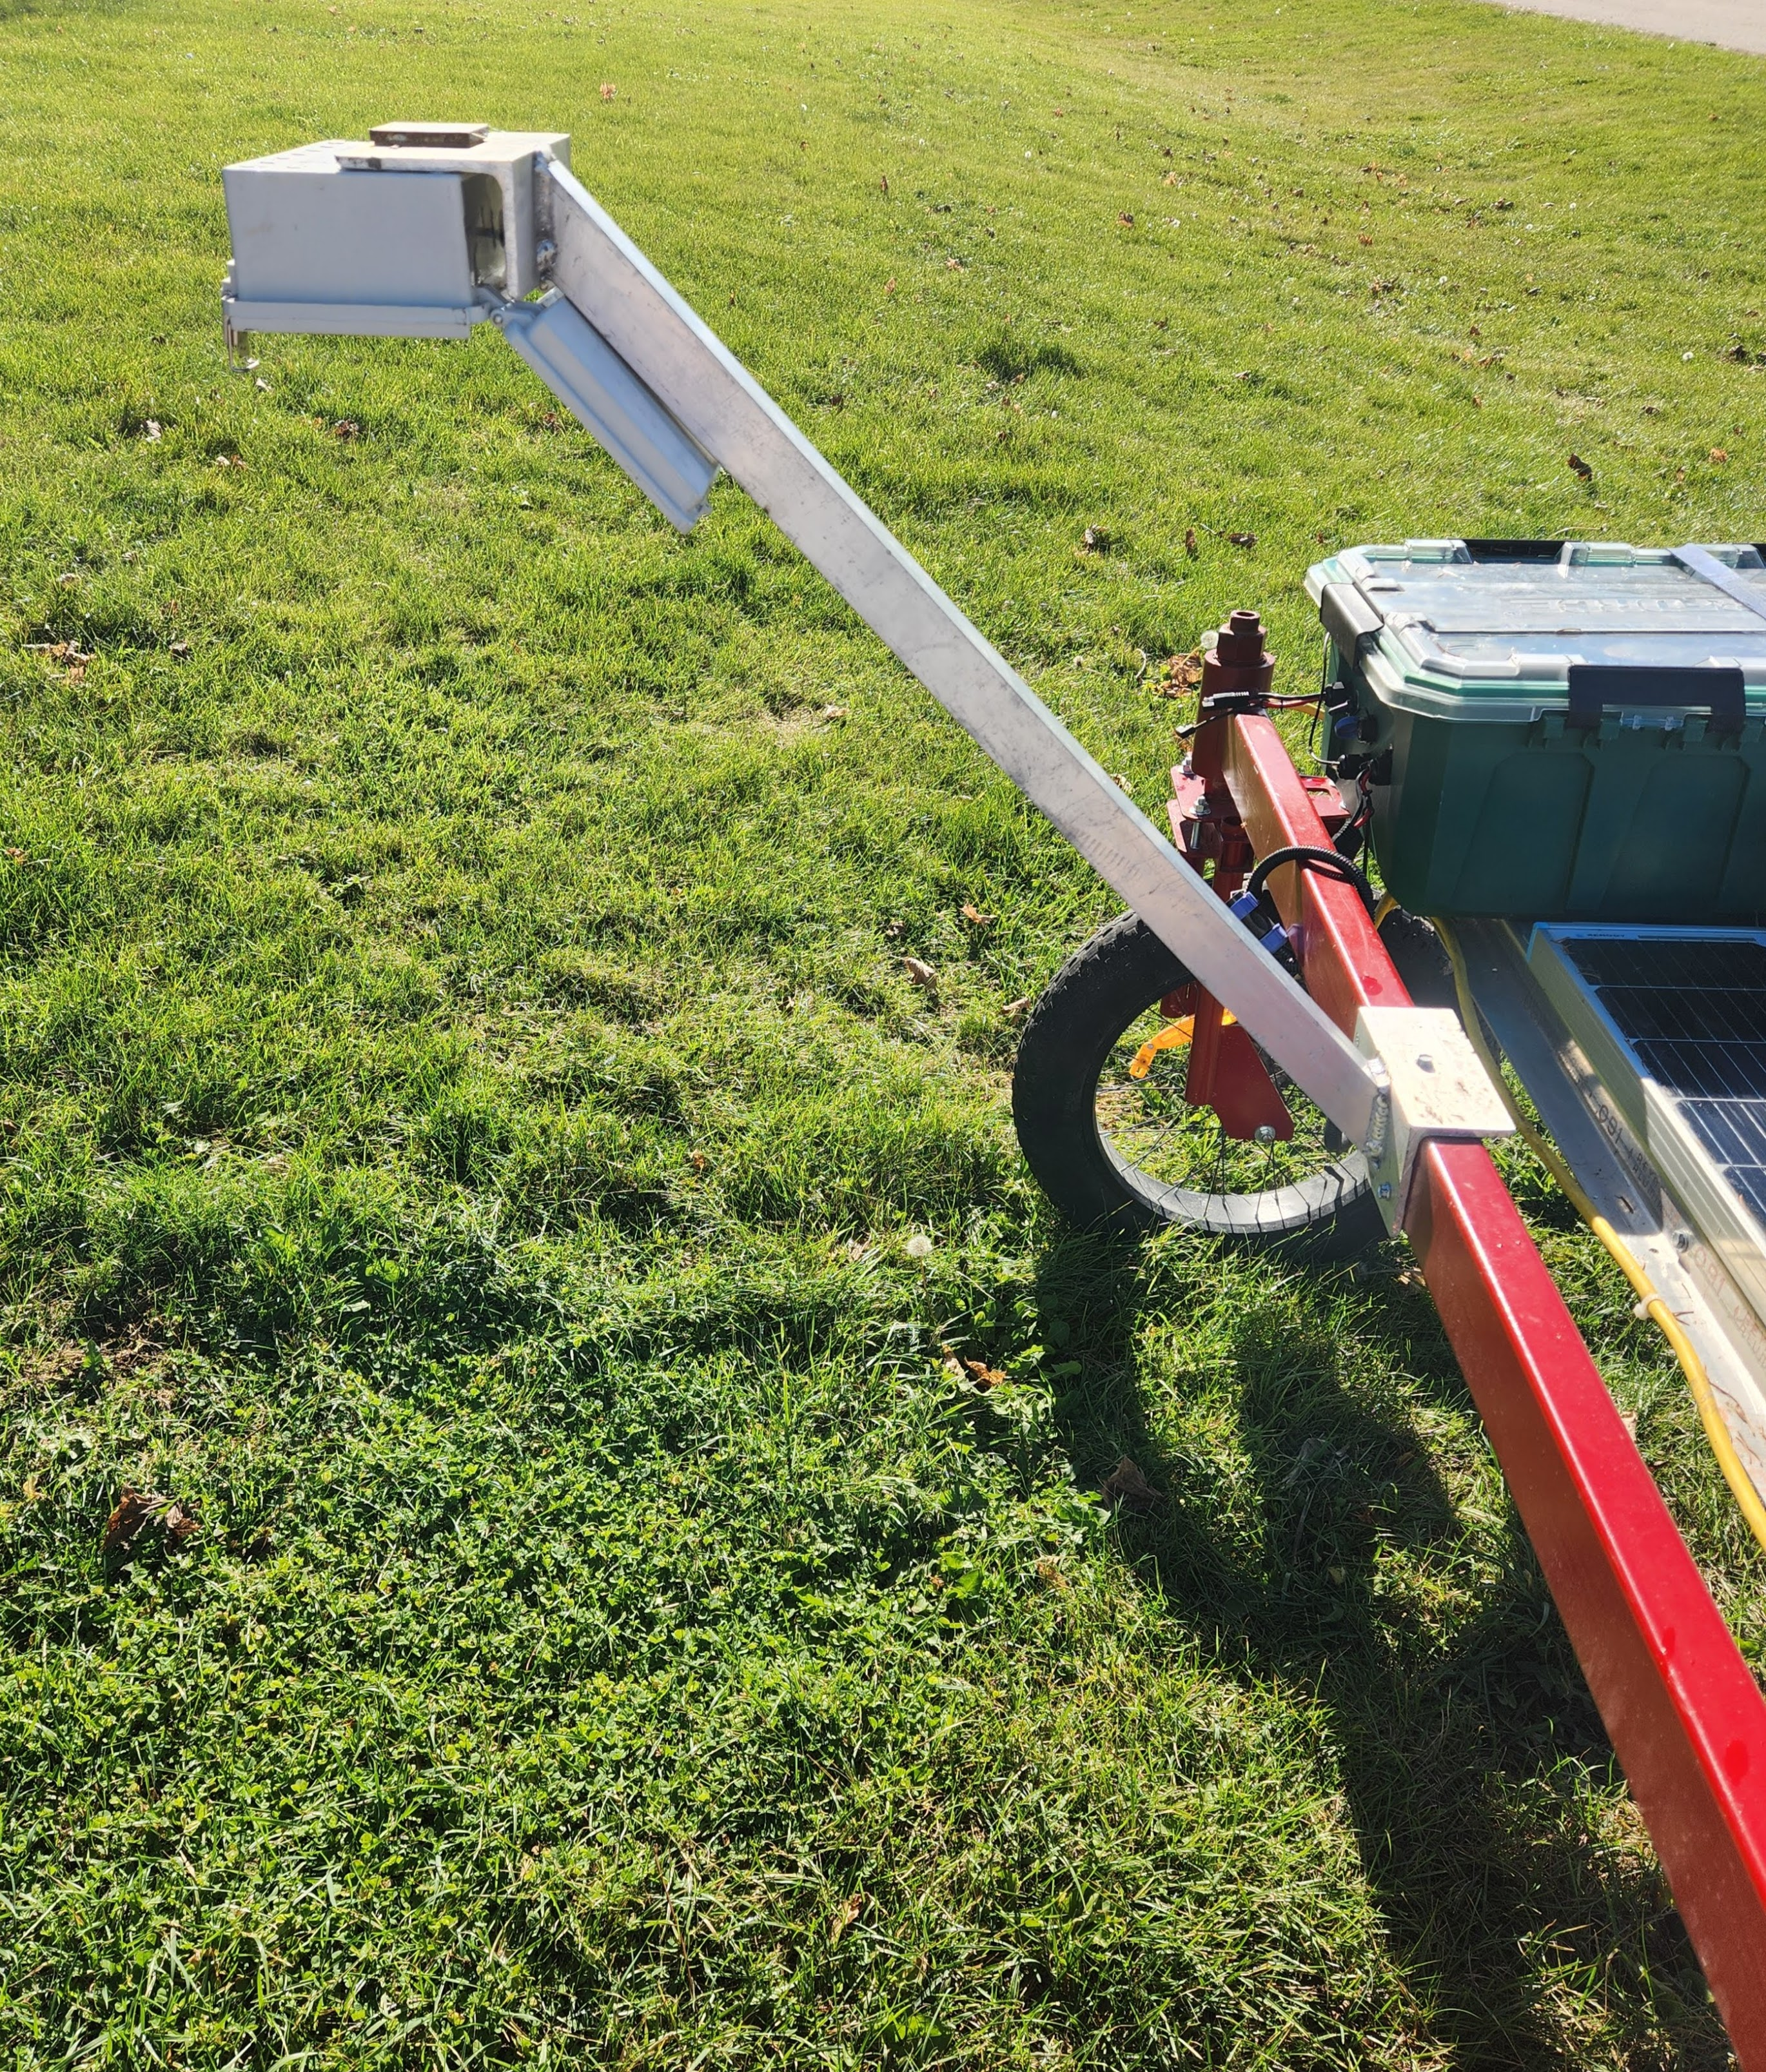
\includegraphics[width=\textwidth]{images/Camera Mounting.jpg}
    \caption{Remote Camera Mount}
    \label{fig:CamMount}
  \end{subfigure}
  \caption{Shadow mitigation strategy. (a) Operating when the solar elevation roughly matches the camera field of view minimizes casting of shadows into the plot. (b) A forward, elevated camera mount places optics ahead of the chassis so any residual shadows fall outside the FOV area. Together these choices improved mask quality and reduced false detections.}

  \label{fig:ShadowMit}
\end{figure}


\subsection{Electronics and Control}

After the completion of the hardware to be used on the sensing platform, the electronics and power system were next selected and implemented.

Current agricultural robotics commonly rely on either electrical or hydraulic power depending on the tasks performed. Hydraulic systems are typically of higher power output and often coupled to internal combustion engines as primary movers. This increased power makes them well suited for and used in seeding and weeding or tilling operations \cite{vahdanjoo_operational_2023}. Lower power systems that typically see use in imaging or crop sensing are often powered by electrical systems as this simplifies maintenance and increases field endurance as they can often be supplemented with recharging areas or solar power \cite{quaglia_design_2020}

For our design, a robust and efficient system is required due to the challenging conditions seen in the cranberry bog the robot would be operating. A particular focus was put onto both heat and water resistance due to the season of sampling, mid to late summer, as well as the use of irrigation in the field. For reasons discussed above, an electrical power system was selected. Thanks to recent advancements, the availability of lithium-ion batteries has greatly improved and is commonly used on other agricultural robotic platforms. \cite{ghobadpour_off-road_2022} A self-contained system that integrates both the lithium cells as well as a battery management system (BMS) was selected; this allowed easier service and replacement if needed. The batteries selected were a Timeusb 12V 50Ah, and (2) battery banks rated at 12 volts nominally were run in series to provide 24 volts to the system as shown in figure~\ref{fig:Battery System}. 

\begin{figure}[!ht]
    \centering
    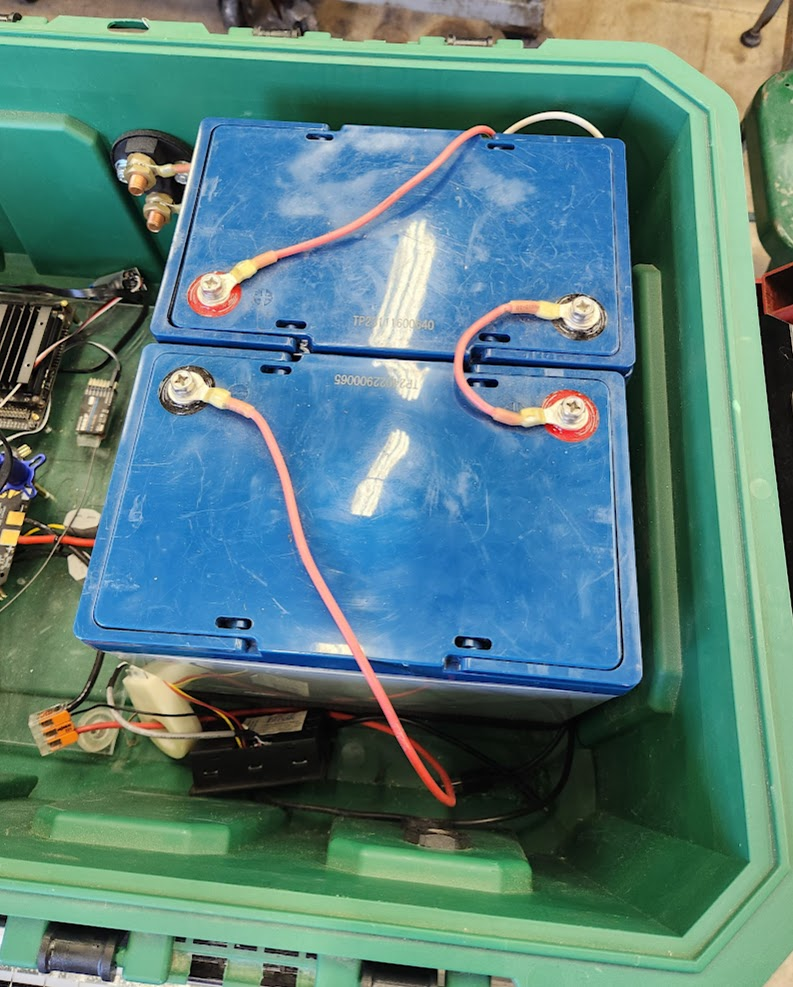
\includegraphics[width=0.5\linewidth]{images/Batteries.jpg}
    \caption{Onboard power system. A LiFePO\textsubscript{4} battery pack in a weather-sealed case supplies power for the controller, compute module, and sensors. The battery pack selected is fully self contained including a internal BMS.}
    \label{fig:Battery System}
\end{figure}

A capacity of 50 amp-hours was selected based on initial calculations using a conservative estimated load of 250 Watts, consumed primarily by the drive motors, at a voltage of 24 volts; nominally, this correlated to a current load of approximately 20.8A.

\begin{equation}
    \frac{250 \, \text{W}}{24 \, \text{V}} = 10.4 \, \text{A}
    \label{eq:power_equation}
\end{equation}

Using this amp loading and an estimated sampling time of 1.5 hours for 360 plots with a sample interval of 15 seconds per plot gave a total energy usage of 15.6 amp-hours, at a nominal voltage of 24 volts this equates to approximately 375 W-hours. The total energy stored by the battery system is approximately 1200 W-Hours. This additional capacity also allows for future expansion and inclusion of additional sensors that may require additional power during operation. In addition to the power storage of the batteries, a solar panel was fitted that provided a maximum of 100 watts to the system. Based on an estimated global horizontal irradiance of 6.1 kWh/m2/day\cite{nrel_pvwatts_2024} and a panel output of 100 Watts the power produced will be approximately 500 W-Hr daily providing the rover with enough energy to fully recharge the energy lost during sampling.

\begin{figure}[!ht]
    \centering
    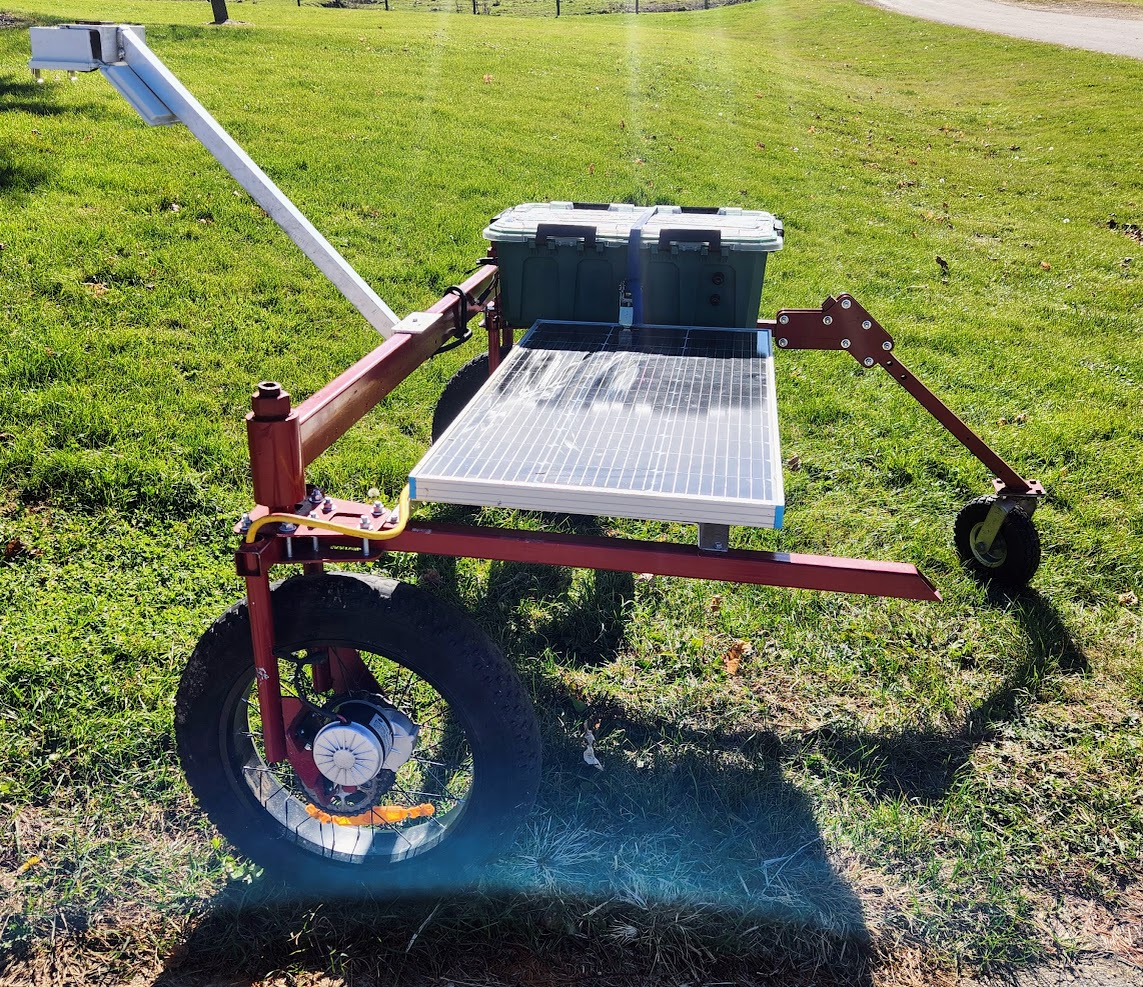
\includegraphics[width=0.5\linewidth]{images/Solar Panel.jpg}
    \caption{100\,W solar replenishment on rover. A panel mounted above the chassis slowly charges the main pack during idle and low-load transits, extending run time across multi-hour sampling sessions.}
    \label{solar-panel}
\end{figure}

The next component selected was the physical ground drive system. Again, multiple options were evaluated before selection. For the ground engaging components, the systems considered were a continuous rubber track or a wheeled drive. While tracks provided decreased ground pressure and improved tractive force, there was concern that turning may disturb the trackways between plots, and it was determined to use 2 20" diameter 4" wide bicycle wheels as the primary ground engaging component. For propulsion, 2 brushed 250W motors, one on each wheel, were used and connected via a chain drive as shown in Figure~\ref{fig:Wheel and drive}. This drive system was simple and would still allow the gearing between the motor and the wheel to be adjusted.

\begin{figure}[!ht]
    \centering
    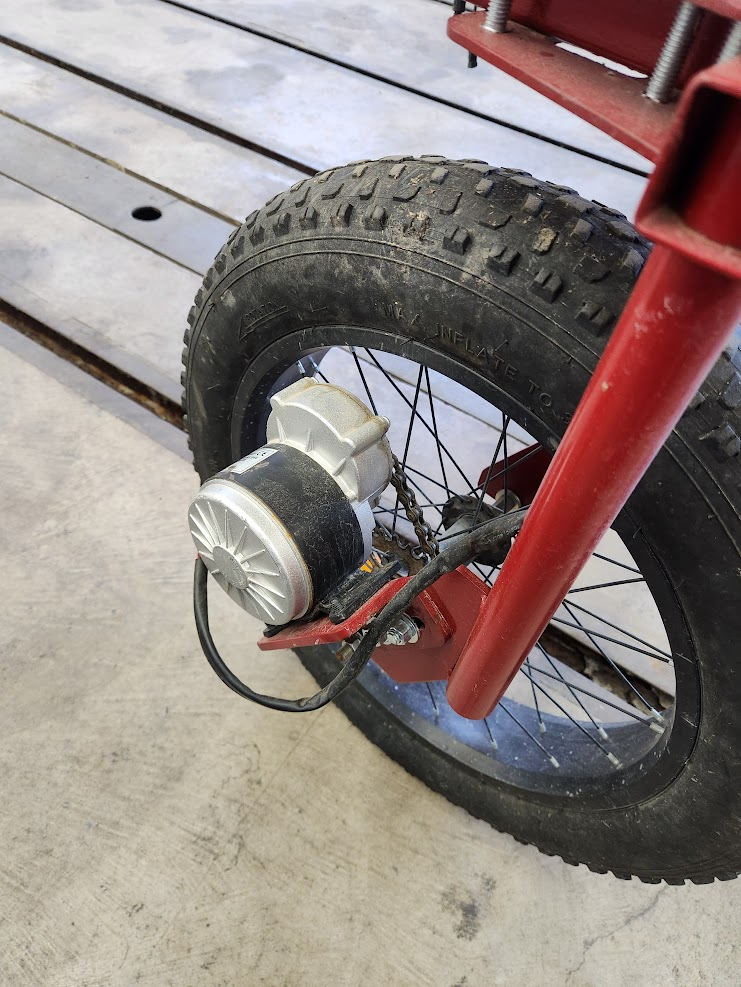
\includegraphics[width=0.5\linewidth]{images/Drive Wheel.jpg}
    \caption{Drive wheels and chain transmission. Two 20\,in pneumatic bicycle wheels driven by 250\,W brushed motors provide traction on soft sand and organic matter typical of cranberry beds. The simple chain reduction allows quick gearing changes to trade speed for torque as needed.}
    \label{fig:Wheel and drive}
\end{figure}

After specifying and assembling all the physical components, the electronic control system was required. Again, reviewing current offerings and maintaining a focus on using commercially available components led to the selection of a consumer-based flight control system. A CubePilot (CubePilot, Australia) flight controller (FC) was selected and mounted to a CubePilot Kore Carrier Board. This system was desirable due to its including many of the necessary auxiliary systems such as a breakout connector for sensors and general-purpose input/output (GPIO) headers.

\begin{figure}[!ht]
    \centering
    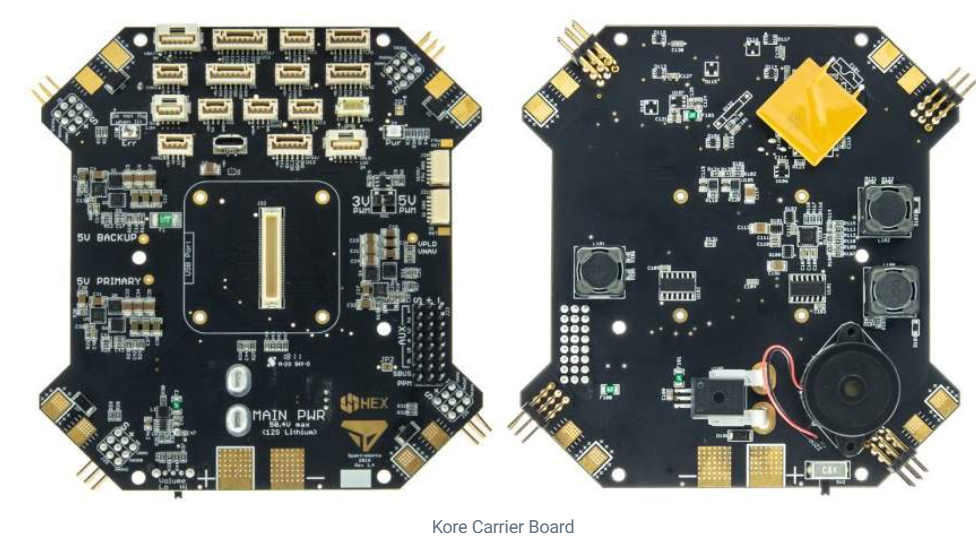
\includegraphics[width=0.5\linewidth]{images/Kore Carrier.png}
    \caption{CubePilot Kore carrier board. The board consolidates power management, sensor breakouts, and GPIO headers for the CubePilot flight controller used here as the rover’s navigation and I/O computer. This off-the-shelf stack reduced custom wiring and improved reliability.}
    \label{fig:Carrier board}
\end{figure}

Multiple solutions were considered for primary navigational data, including vision-based, laser-guided, and RTK GPS. After evaluation, RTK GPS was found to be the most suitable due heavily to its ease of implementation as well as accuracy to sub-inch levels. Two systems were used to increase redundancy. The primary system was a system produced by Emlid (Emlid, Hungary) Reach M2 UAV RTK Kit. This kit includes a base station that uses a Long Range (LoRa) radio unit to send correction data to the rover as shown in Figure~\ref{fig:Local Corection RTK}.

\begin{figure}[!ht]
    \centering
    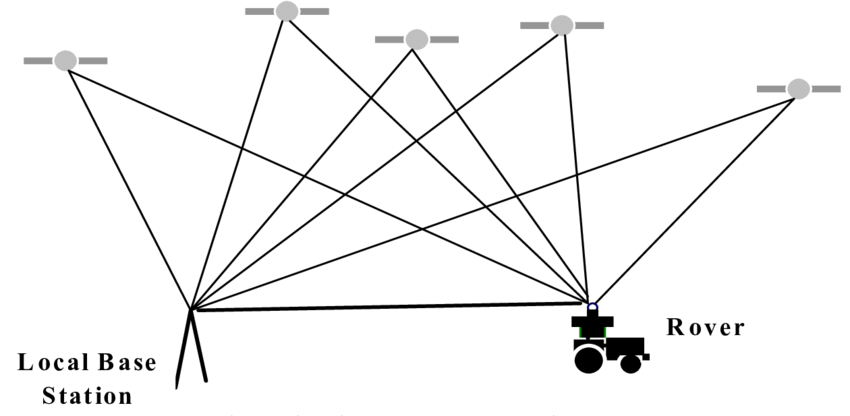
\includegraphics[width=0.5\linewidth]{images/RTK-GPS.png}
    \caption{RTK system with local base station. An Emlid Reach M2 base broadcasts RTCM corrections over LoRa to the rover receiver, enabling sub-inch positioning for plot alignment. This mode was used when on-site base setup was feasible and radio line-of-sight was reliable.}
    \label{fig:Local Corection RTK}
\end{figure}

The second system is a SparkFun GPS-RTK2 development board (SparkFun, USA) that uses a ZED-F9P module by UBlox (UBlox, Switzerland). This system uses a Networked Transport of RTCM via Internet Protocol (NTRIP) service for corrections provided by the Wisconsin Continuously Operating Reference Station (WISCORS) operated by the Wisconsin Department of Transportation. The WISCORS system works by collecting and combining atmospheric correction data from 115 stations throughout the state and providing correction data through a web application available to the public\cite{wisconsin_department_of_transportation_wiscors_nodate}. 

\begin{figure}[!ht]
    \centering
    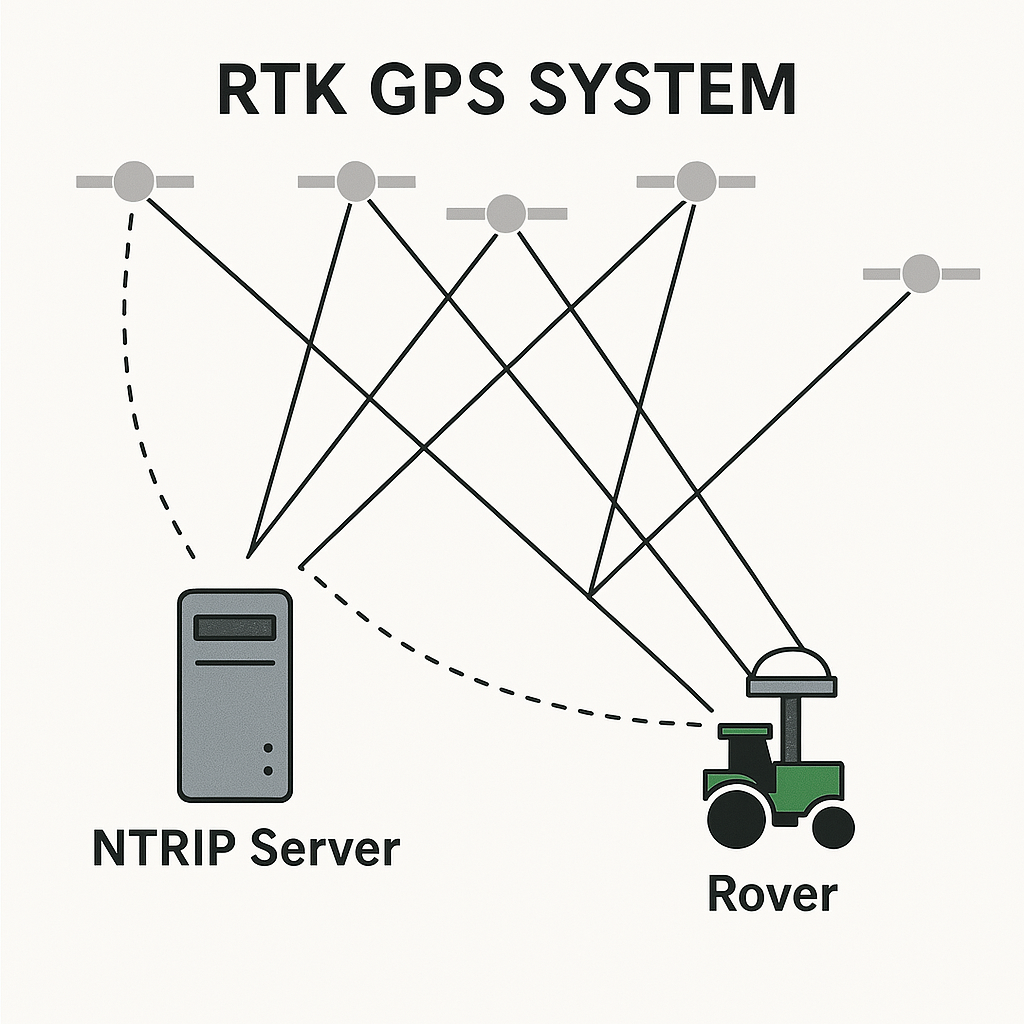
\includegraphics[width=0.5\linewidth]{images/Ntrip.png}
    \caption{RTK via NTRIP corrections. A ZED-F9P receiver on the rover obtains state-wide corrections from the WISCORS network over internet accessable data. This configuration provided a no-base alternative with comparable accuracy when infrastructure access was available.}
    \label{fig:NTRIP RTK}
\end{figure}

To control and program the physical rover unit, a ground station was used. We used the Open Source Software package Mission Planner ver 1.3.82, maintained by the ArduPilot team \cite{ardupilot_mission_nodate}. This allowed us to both program parameters into the rover used in navigation and control, as well as upload specific missions used for path planning and waypoint creation during the data collection.

\begin{figure}[!ht]
    \centering
    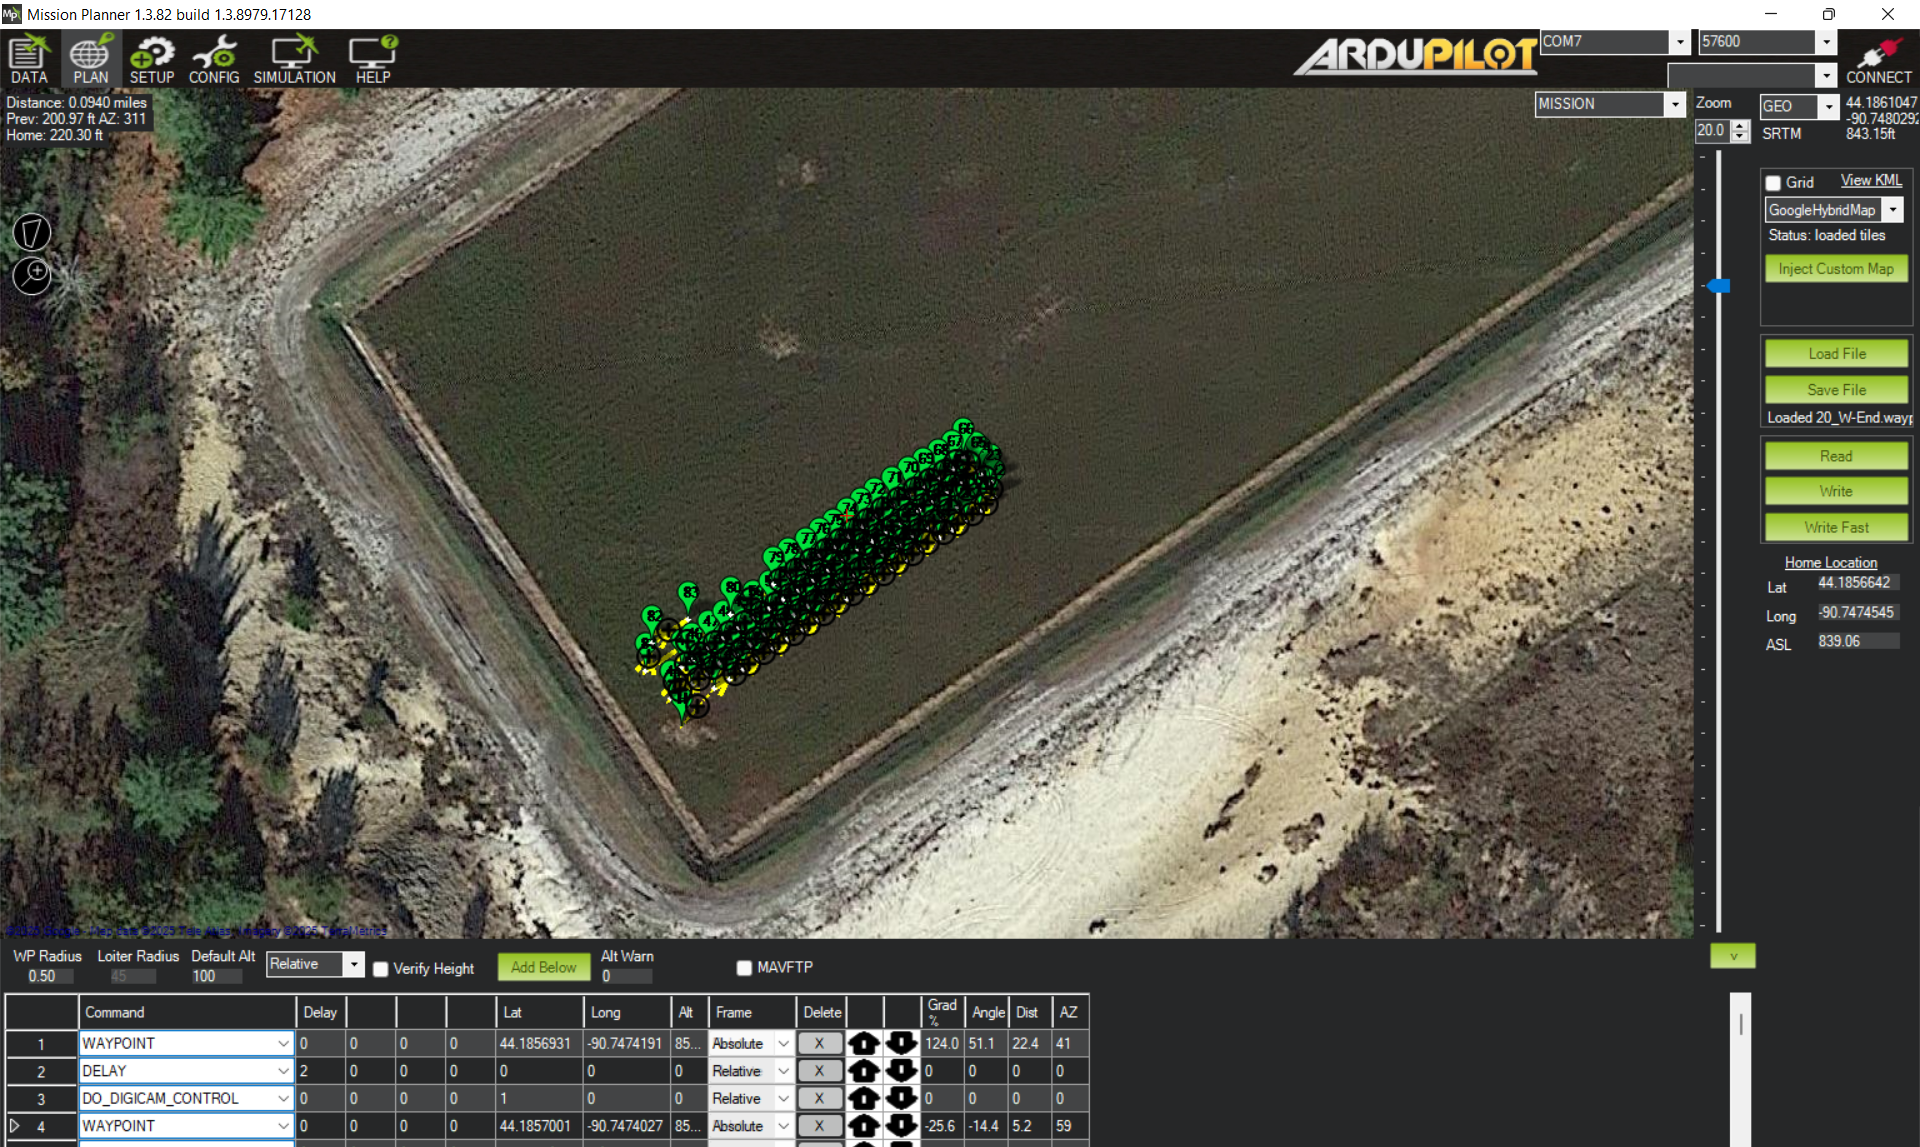
\includegraphics[width=0.5\linewidth]{images/Mission Planner.png}
    \caption{Mission Planner ground-station interface. The operator configured rover parameters, uploaded waypoint missions, and logged GNSS status through this interface. Using a repeatable mission file ensured consistent plot coverage across collection days.}
    \label{fig:Mission Planner}
\end{figure}

\section{Testing}

Plots were surveyed 2 times, once with a handheld RTK receiver placed at the center of each plot on the East End of the field and once using the rover. To use the rover for surveying, it was manually piloted to be centered over the plot and then triggered to record its position as a way-point in the mission planner software. This technique was able to produce a high-quality map of desired way-points without additional processing and removed potential errors during translation between hardware setups.

\begin{figure}[!ht]
    \centering
    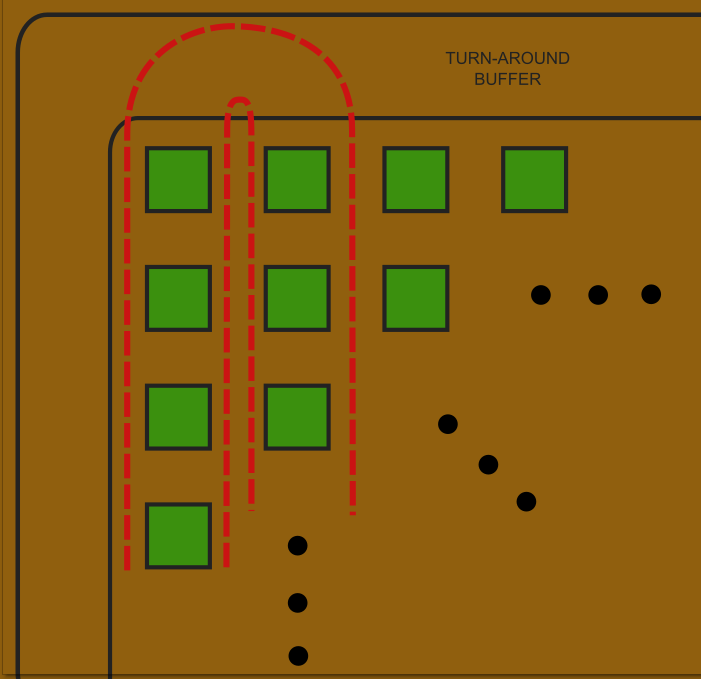
\includegraphics[width=0.5\linewidth]{images/TurnAround.png}
    \caption{Robot path navigation for plot coverage. Waypoints were centered over each plot; turns used buffer lanes to avoid driving through imaged plant canopies. The repeatable path minimized trampling, reduced navigation time, and kept imaging geometry consistent.}
    \label{fig:path}
\end{figure}

\begin{figure}[!ht]
    \centering
    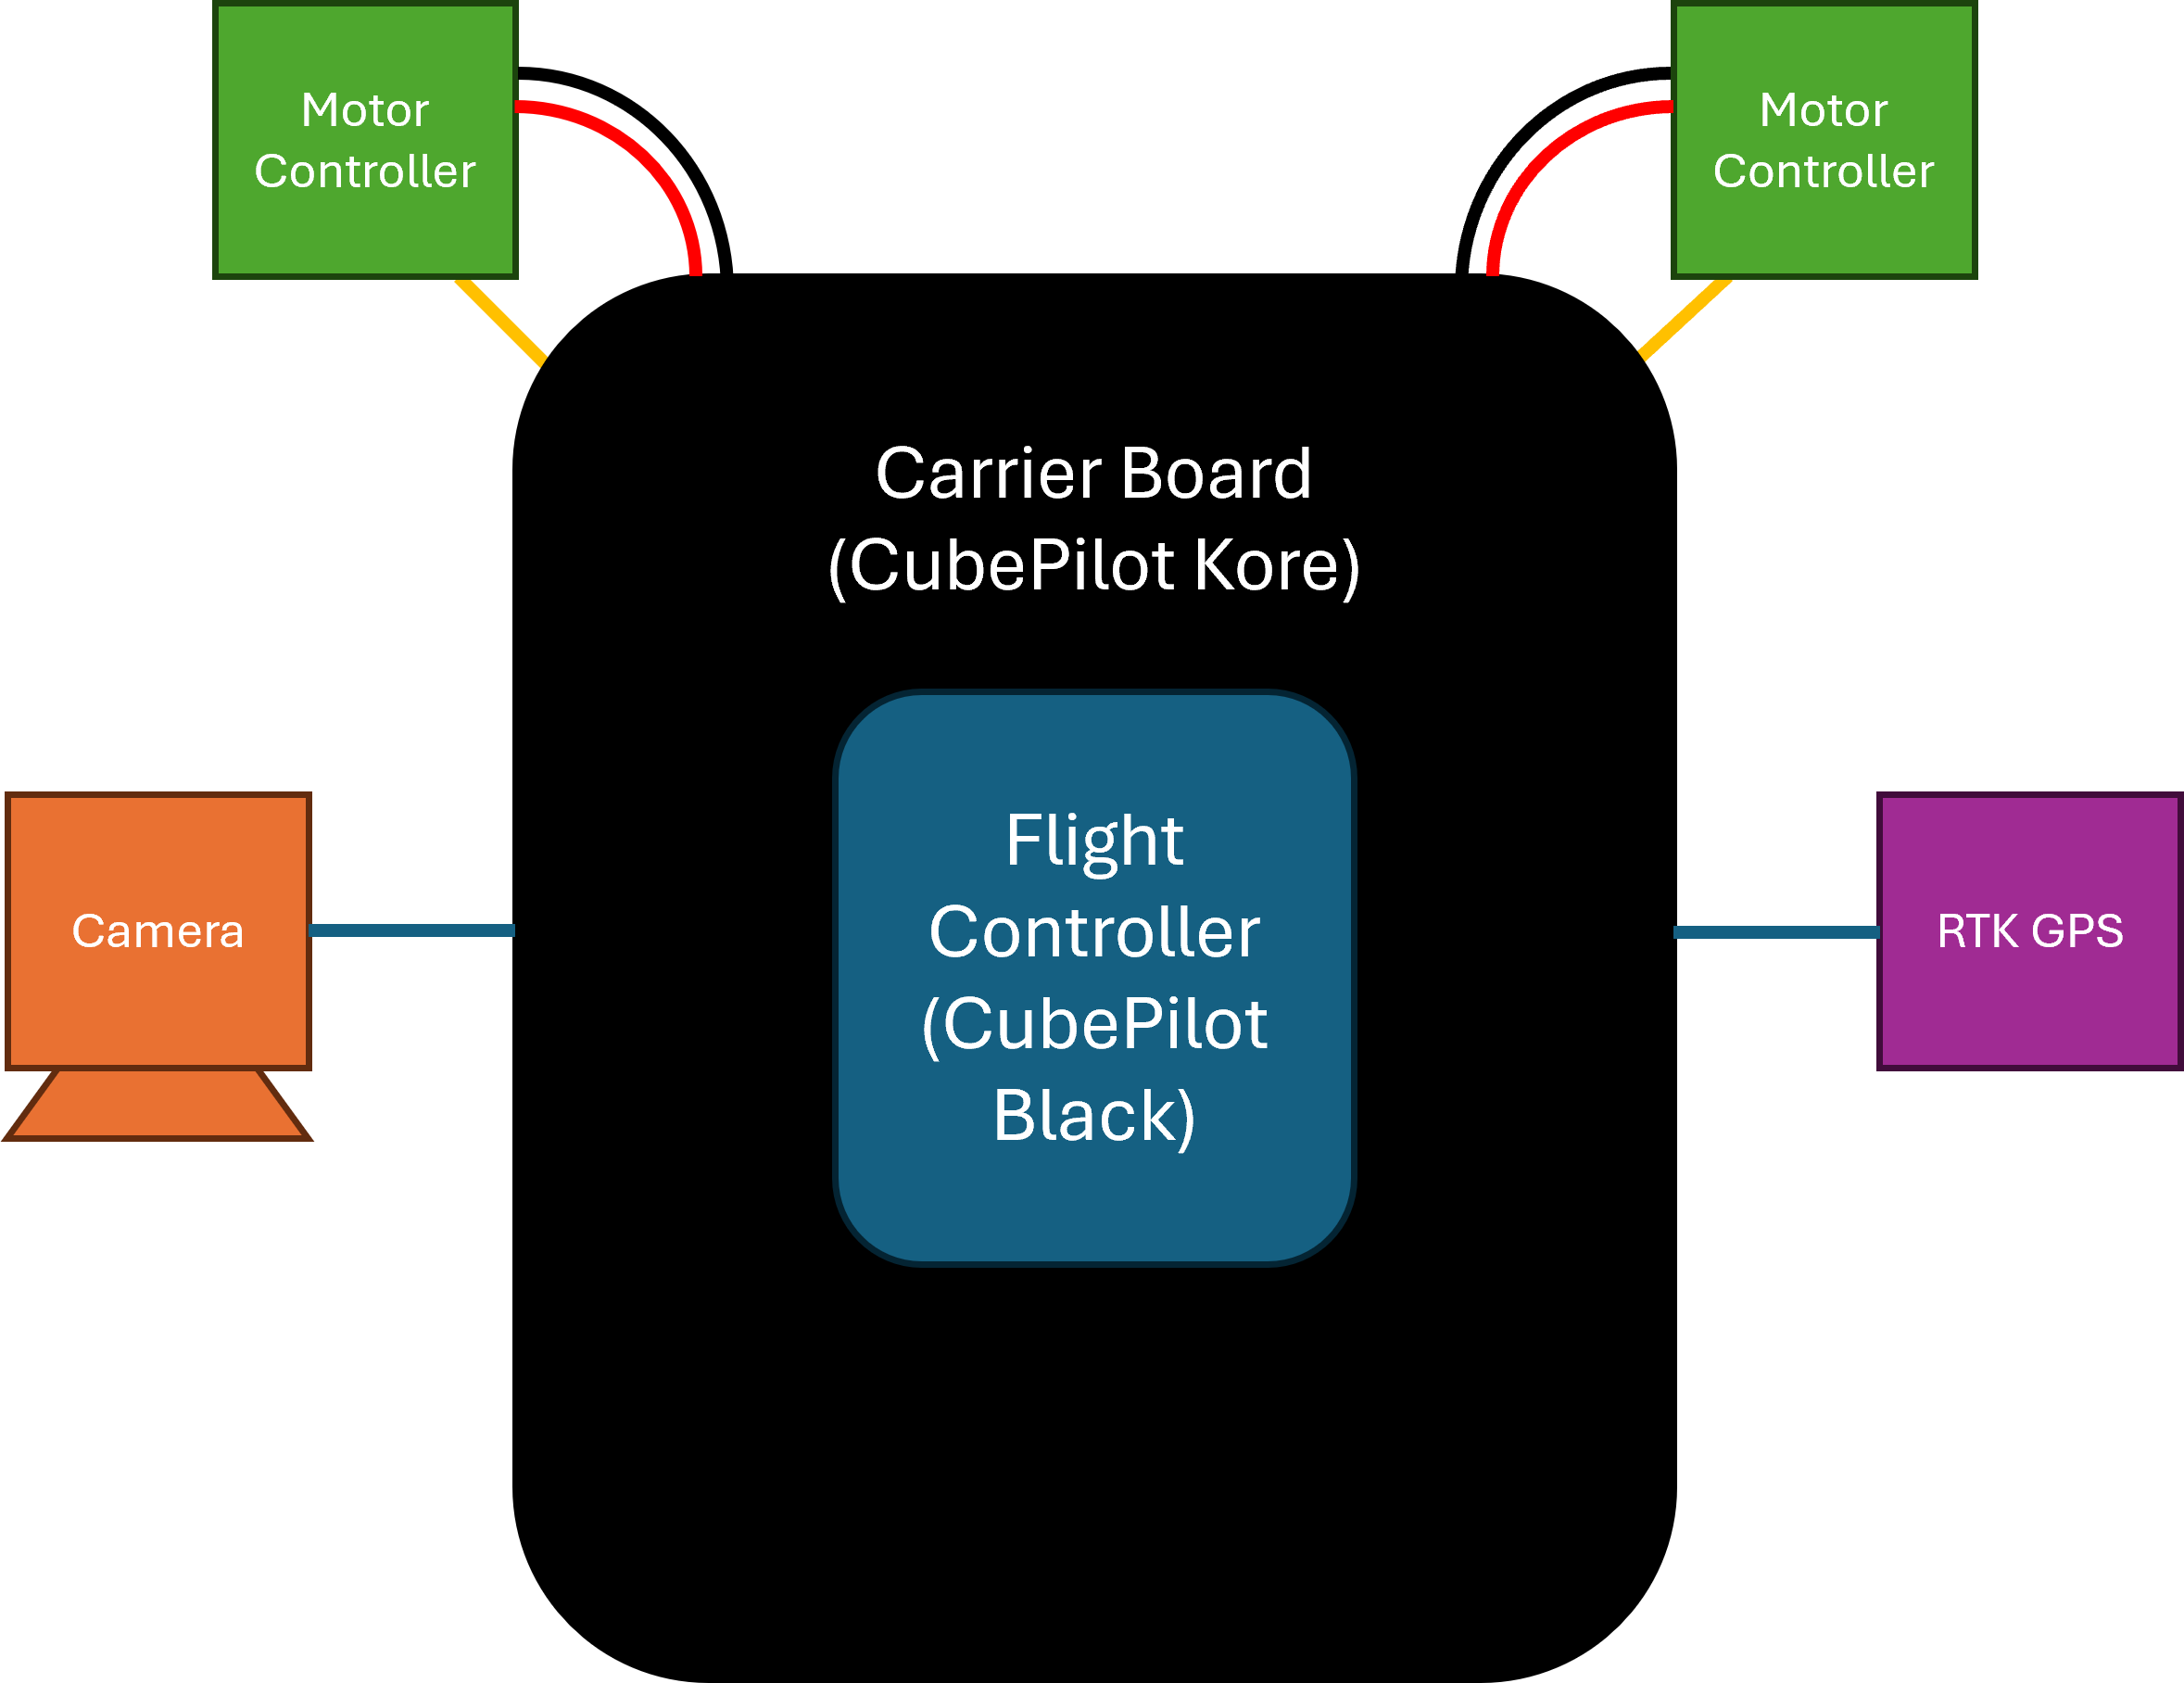
\includegraphics[width=0.75\linewidth]{images/Block_Dia_1.png}
    \caption{System block diagram. Sensors (RGB camera, GNSS/IMU) feed the controller, which handles mission execution and time-stamped image capture. Power distribution, storage, and telemetry are separated into modular subsystems to simplify troubleshooting and field swaps.}
    \label{fig:Block Diagram}
\end{figure}

\section {Bill of materials}

A complete list of materials used, as well as sources and prices at the time of purchase, is listed below.


\begin{table}[!ht]
    \centering
    \caption{Bill of Materials}
    \label{tab:bom}
    \footnotesize
    \begin{tabular}{r l l l c}
        \toprule
        \textbf{Item} & \textbf{Part} & \textbf{Description} & \textbf{Source} & {\textbf{Price (\$)}} \\
        \midrule
        1  & CubePilot Black   & Flight Controller        & IR-LOCK      & 800 \\
        2  & CubePilot Kore    & Carrier Board            & IR-LOCK      & 300 \\
        3  & SparkFun RTK SMA  & RTK GPS Receiver         & IR-LOCK      & 260 \\
        4  & Pololu G2 18v17   & Motor Driver             & Pololu       & 45  \\
        5  & 20 inch Wheels and Hub & Drive Wheel         & Local Source & 85  \\
        6  & Solar Panel       & 100W Renogy Panel        & Amazon       & 125 \\
        7  & Battery           & 50 Ah 12V Battery        & Amazon       & 185 \\
        8  & RC Remote Control & RadioLink T8S            & Amazon       & 55  \\
        9  & Steel             & Tube and Plate for Frame & Local Supply & 180 \\
        10 & Enclosure         & Masterforce 5 gal Tote   & Menards      & 22  \\
        \midrule
        \multicolumn{4}{r}{\textbf{Total}} & {\bfseries 2057} \\
        \bottomrule
    \end{tabular}
\end{table}

\newpage


\section{Conclusion}

Overall the system proved to be robust and able to operate well in real-world field conditions. Traction of the drive system and drive power were more than satisfactory. Additionally, the requirement to operate over extended periods without recharging was found to be well exceeded, with the rover able to complete over three full field samplings without any additional off-site or solar charging. The physical structure of the rover was updated to improve performance as well as increase reliability. Steering was changed from having two systems, rotatable drive wheels and differential steering, to exclusively using the differential steering. While differential steering has been used in many agricultural robots \cite{veiros_multitask_2022} the use of two drive wheels with passive caster wheels for stability offers notable improvements in agility in addition to a decreased risk of crop damage. The primary difficulty found was in accurately navigating between plots and then pivoting at the end of rows in order to move to the next row without excessive navigation over existing crop. This issue could be mitigated by utilizing the rows of buffer areas surrounding the test areas as shown in Figure~\ref{fig:path}. Additionally, damage to any crop or fruit was reduced due to the rover's light weight combined with the large footprint of the pneumatic tires. To improve navigation accuracy, it was determined that further decreasing the gearing between the motors and drive wheels would help to lower the operating speed and allow the motion controller to better correct for errors due to uneven terrain; additionally, the inclusion of closed-loop control over the drive motors may decrease overshoot while maneuvering.

This work showed the potential of an automated image collection system that was cost-effective while still being robust enough for season-long use. The 2-wheel drive configuration exhibited good maneuverability while also simplifying the overall machine layout and minimizing damage to the crop or field due to skidding.  Improvements to the navigation system would increase the usability of the system and allow for the addition of further sensors as well as manipulators to interact with crops as needed.

\newpage

\section{References}

\printbibliography[heading=none]



\chapter{Cranberry Flower Detection from Ground Imagery for Early Yield Prediction}
\section{Abstract}

\begin{singlespace}
    
The current approach used for the prediction of yields in cranberry production relies on selecting and handpicking a 300~mm~$\times$~300~mm quadrat and then extrapolating this result. In addition to being a time-consuming manual process, this system can often lead to variation in measurements due to human error as well as to spatial variation throughout the cranberry bed \cite{pozdnyakova_estimation_2002}.

This study applied machine learning algorithms in coordination with the automated image capture and detection, classification, and counting of cranberry flowers using high-resolution images. 626 genetic plots were imaged from June to August 2024 to capture peak flowering timing and were hand-annotated to create a training dataset of 1478 images with 51,732 individual annotations. These data were then used to train four machine learning models, YOLOv11, YOLOv12, Roboflow 3.0, and RF-DETR. These models were able to accurately identify, classify, and count various stages of flowering. The highest performing model, considering both accuracy and CPU latency, was YOLOv12 offering the best trade-off (mAP@0.50 = 69.3\%, F1 = 71.9\%) despite RF-DETR achieving the highest mAP.

Using this trained model, we then analyzed thirty plots. Plots were split into two groups based on genetic variation, one set of Stevens plots representing a control group and one set of Experimental variations with differing genetic traits. Plots were sampled three times at 5-day intervals from the end of June to early July, representing peak flowering timing. Using these images, we detected multiple stages of flower development and recorded flower counts per plot over the three imaging sessions. Using this new dataset, we compared the temporal flowering patterns of the two groups. Plots were also sampled in the standard method on two separate days to generate a ground truth dataset reporting fruit count and yield. Across 30 plots, total flower count moderately predicted total berry count in Experimental hybrids \rnp{0.68}{20}{= .001}.

This workflow demonstrates the potential for an automated system that can image cranberry flowers, detect and classify the blooms, and use these data to predict berry production. Although the workflow requires further development, the use of such a system would prove invaluable to growers as it enables yield signals weeks to months before harvest, informing harvest planning and in-season management.

\end{singlespace}

\section{Introduction}

Cranberry (\textit{Vaccinium macrocarpon} Ait.) is a high-value North American crop that thrives in cool, temperate climates with acidic, sandy soils and abundant freshwater sources \cite{sandler_cranberry_2008}. Wisconsin produces roughly 62\% of U.S. cranberries \cite{usda-nass_cranberries_2024}, making the crop economically and ecologically central to the state. Commercial production typically occurs in diked marshes (“bogs”) that can be flooded and drained for management and harvest; beds are constructed in low-lying areas and lined with peat, sand, and gravel to support the crop’s shallow root system. Because these engineered wetlands often occupy large, remote tracts with limited technological infrastructure, high-speed internet or even cellular coverage can be unreliable. Cranberries also require a long growing season with warm summers and cold winters to satisfy dormancy requirements \cite{ellwood_cranberry_2014}. Intensive water management—leveraging flooding for frost protection, weed control, and wet harvesting—adds operational complexity. These field conditions challenge conventional management and complicate the deployment of robotics and other precision-agriculture tools at scale. In addition to field conditions, the remote nature of most cranberry operations and connectivity constraints underscore the need for robust, field-deployable, and—ideally—edge-computing ML solutions.

Recent advances in image-based machine learning have begun to influence crop management by improving monitoring, analysis, and decision-making. In large-scale systems, ML supports crop health surveillance, weed and pest detection, yield prediction, and precision input application \cite{akiva_vision_2022}. High-resolution imagery from drones, satellites, and field cameras, paired with deep models such as convolutional neural networks (CNNs), enables early disease detection, real-time assessment, and targeted resource allocation. AI-driven weed detection improves herbicide precision \cite{wendel_self-supervised_2016}, while yield-estimation models leverage plant density, biomass, and environmental co-variates to optimize harvest planning \cite{ni_deep_2020}. Automated phenotyping accelerates breeding by quantifying traits such as berry size and shape \cite{diaz-garcia_image-based_2018}.

In specialty crops like cranberries, accurate detection of flowering stages and early fruit set is critical for yield prediction \cite{coombe_development_1980}, yet current field monitoring is labor-intensive, error-prone, and slow to deliver actionable feedback \cite{pozdnyakova_estimation_2002}. These challenges highlight the need for image-based approaches that can accommodate field variability and function reliably under real-world conditions.

This study investigates deep learning and computer vision for flower and early-fruit detection in cranberry to improve yield prediction and support precision management. Using high-resolution, ground-based imagery collected by an autonomous platform, we develop and evaluate a workflow for detection, classification, and counting. Our pipeline utilizes CNN-based architectures to accurately isolate flowers within dense canopies and address occlusion and morphological variability \cite{ghosh_understanding_2019}.

To enhance robustness, we assembled a large, annotated dataset and applied data augmentation (rotation, flipping, contrast adjustments). Beyond flower counting, we explore predictive links between floral dynamics, pollination success, and subsequent yield by integrating temporal image sequences with environmental data \cite{brown_fruit_2006,parent_current_2021}. These experiments test whether early-season imagery can forecast yield and inform irrigation, nutrition, and pollination strategies in near real-time. The novel deliverables from this project are as follows:

\par\medskip 

\begin{spacing}{1}
\begin{enumerate}[label=(\arabic*), leftmargin=2em, labelsep=0.6em, align=left,
                  itemsep=8pt, parsep=0pt, topsep=0pt, partopsep=0pt]
  \item A robust imaging platform and modeling pipeline for detecting cranberry flowers and early fruit, classifying detections, and producing counts.
  \item Creation of a dataset and training protocol designed for field variability, improving generalization across beds, cultivars, and imaging conditions.
  \item An initial demonstration that temporal flower counts correlate with early yield prediction.
\end{enumerate}
\end{spacing}

While this study focused on cranberries, the methodology could be expanded to other specialty crops that require precise floral monitoring \cite{estrada_deep_2024}.

\section{Materials and Methods}

In order to develop a high performing ML model, a large yet consistent dataset of images is required. In this study, we collected 3,308 images through manual imaging and the use of an automated ground rover at the Wisconsin Cranberry Research Station in Black River Falls, WI. The images were collected over a three month period from June 2024 to August 2024. These dates were chosen in order to capture the peak flowering dates as well as early stage fruit development \cite{sandler_cranberry_2008}. Images were collected with a Canon PowerShot A810 (Canon U.S.A, USA) with a full resolution of 4608 $\times$ 3456, giving a 16 megapixel image size. Images were captured at a height of 1500 mm and with the field of view adjusted to capture an area approximately 1200 mm $\times$ 1700 mm. This FOV and image resolution gave a ground sampling distance (GSD) of approximately 0.37 mm/px. This resolution was chosen as a typical blossom was found to be approximately 6.3 mm to 9.5 mm \cite{diaz-garcia_image-based_2018}, with some features such as individual petals being smaller. The combination of flower size and GSD ensured approximately 15-20 pixels per flower. Images were captured using natural lighting in the early afternoon to provide minimal self-shadowing and to avoid shadowing from the image collection platform. 

After images were acquired, they were cropped to a resolution of 640 $\times$ 640 px, resulting in a sample space of approximately 56,000~\(\text{mm}^2\). This size was chosen to aid in manual labeling. It was found that reducing the number of flowers to be annotated would allow annotators to more effectively visually scan the image for missing or mislabeled annotations. Reducing image size also allowed multiple samplings per image as needed to increase the number of training images. Images were also renamed at this time to add the plot number that the sample was taken from as well as the date. After pre-processing, the images were uploaded to Roboflow for annotation and training. During cropping, overlapping tiles were not used to avoid double counting, and only one image per plot/date was used.

Annotating the collected images for machine learning involved labeling images to create a training dataset used to classify features effectively\cite{ghosh_understanding_2019}. The purpose of the models in this project will be to detect flowering, classify the objects detected, and count instances of features. Relevant categories for this paper will be Early Blossoms (EB), Late Blossoms (LB) and Early Fruiting (EF). The Segment Anything Model (SAM)\cite{kirillov_segment_2023} was used to create masks and assign labels to images. SAM was used to assist annotation only; all reported results are object detection (bounding boxes), not segmentation. Special attention was given to complex scenarios, such as overlapping objects and occlusions, to ensure accurate representation. A total of 51,732 annotations were labeled across the three classes.

The full dataset was then reviewed by one annotator to ensure consistency and quality. Once validated, annotations are used to train ML models. Data were split into 70\% for training, 20\% for validation, and 10\% for testing. Additionally, splits were performed by plot and date to ensure the same plot/date never appeared in different splits, preventing near-duplicate content leakage. Our models were trained using Roboflow's NVIDIA-based GPU clusters\cite{dwyer_roboflow_2024}. Four models were used in the ML training: YOLOv11, YOLOv12\cite{jocher_ultralytics_2023}, Roboflow 3.0 (RF3), and RF-DETR\cite{deng_cross-domain_2024}.

After training, the performance was measured using mAP, Precision, Recall, and F1-score. These metrics are widely used in object detection and classification tasks to provide a comprehensive assessment of model performance\cite{rainio_evaluation_2024}.

\begin{align}
\text{Precision} &= \frac{TP}{TP+FP} \\[1ex]
\text{Recall} &= \frac{TP}{TP+FN} \\[1ex]
\text{F1-score} &= \frac{2 \times \text{Precision} \times \text{Recall}}{\text{Precision} + \text{Recall}}
\end{align}

where TP, FP, and FN denote true positives, false positives, and false negatives.

In addition to the performance benchmarks listed above, a script was created to measure inference time for the 4 selected models. The python-based script would load each model individually, run a desired number of "warm-up" inferences, and then measure the per-image inference time on a desired set of images a chosen number of times and return the results.


The best performing model was then used to analyze all images collected on a subset of plots during peak flowering season and used to produce a dataset allowing for correlation testing between flower count to yield. Yield ground truth data was gathered on two dates, with the first being on September 12\textsuperscript{th}, 2024, and the second being October 4\textsuperscript{th}, 2024. Harvest was carried out using a standard hand harvesting method of selecting a 300~mm~$\times$~300~mm quadrat and harvesting all the fruit within the boundary. After harvest, the fruit was sorted into samples of good fruit and rotten fruit by plot. Each sample was counted to determine the total number of individual fruit, identified as the Good Count (GC) and Rotten Count (RC), and then weighed to determine the yield of each sample identified as the Good Yield (GY) and Rotten Yield (RY). Thirty plots were sampled during each of the harvests, and plots were split into control plots that contained only the Stevens cultivar and Experimental plots that contained various genetic hybrids. We analyzed flower counts and ground-truth yields to quantify correlations using the SciPy library \cite{virtanen_scipy_2020} paired with the seaborn data visualization library \cite{waskom_seaborn_2021} to determine correlation between flowering timing and count to yield.


\section{Results and Discussion}

Images for training were gathered from June 14th to August 14th, 2024, at the Wisconsin Cranberry Research Station (Black River Falls, WI). Initially, a RealSense D435i (Intel, USA) camera was used; however, the resolution and lighting for the camera resulted in poor-quality images, and these images were not used. For the remainder of the season, a Canon PowerShot A810 (Canon U.S.A., USA) camera was used and provided high-quality images. The list of dates and images collected can be found in Table~\ref{tab:image dates}


\begin{table}[!ht]
    \centering
    \caption{Data Collection Dates}
    \label{tab:image dates}
    \begin{tabular}{cccc} 
      \toprule
      \textbf{Date} & \textbf{Location} & \textbf{Camera System} & \textbf{Images Collected}\\ 
      \midrule
      June 14th & East & Intel RealSense D435i & 266\\ 
      June 17th & East & Intel RealSense D435i & 266\\ 
      June 20th & East & Canon PowerShot A810 & 266\\ 
      June 21st & East & Intel RealSense D435i & 216\\ 
      June 22nd & East & Canon PowerShot A810 & 266\\ 
      June 22nd & West & Canon PowerShot A810 & 284\\
      June 27th & West & Canon PowerShot A810 & 320\\ 
      July 2nd  & East & Canon PowerShot A810 & 266\\ 
      July 2nd  & West & Canon PowerShot A810 & 360\\
      July 31st & East & Canon PowerShot A810 & 266\\ 
      Aug 5th   & East & Canon PowerShot A810 & 266\\ 
      Aug 14th  & East & Canon PowerShot A810 & 266\\
      \midrule
      \multicolumn{3}{r}{\textbf{Total}} & \textbf{3,308}\\
      \bottomrule
    \end{tabular}
\end{table}


After labeling, there were 51,732 annotated features across 1,478 images. The summary of annotation counts and average per image is shown in Table~\ref{tab:dataset-summary} with the distribution shown in Figure~\ref{fig:Annotations per Image}. For model training, the dataset was split into 1,034 training images, 297 validation images, and 147 'held-out' test images.


\begin{table}[!ht]
\centering
\caption{Dataset summary and annotation counts}
\label{tab:dataset-summary}
\footnotesize
\setlength{\tabcolsep}{6pt}

\begin{subtable}[t]{0.45\linewidth}
\centering
\caption{Annotation Counts Per Image}
\begin{tabular}{lr}
\toprule
\textbf{Metric} & \textbf{Value} \\
\midrule
Number of Images         & 1,478 \\
Mean Annotations/Image   & 35.12 \\
Standard Deviation       & 44.46 \\
\bottomrule
\end{tabular}
\end{subtable}
\hfill
\begin{subtable}[t]{0.45\linewidth}
\centering
\caption{Annotation Classes and Counts}
\begin{tabular}{lr}
\toprule
\textbf{Class} & \textbf{Count} \\
\midrule
Early Bloom (EB)  & 1,044 \\
Late Bloom (LB)   & 45,363 \\
Early Fruit (EF)  & 5,325 \\
\midrule
\textbf{Total}    & \textbf{51,732} \\
\bottomrule
\end{tabular}
\end{subtable}
\end{table}



\begin{figure}[!ht]
    \centering
    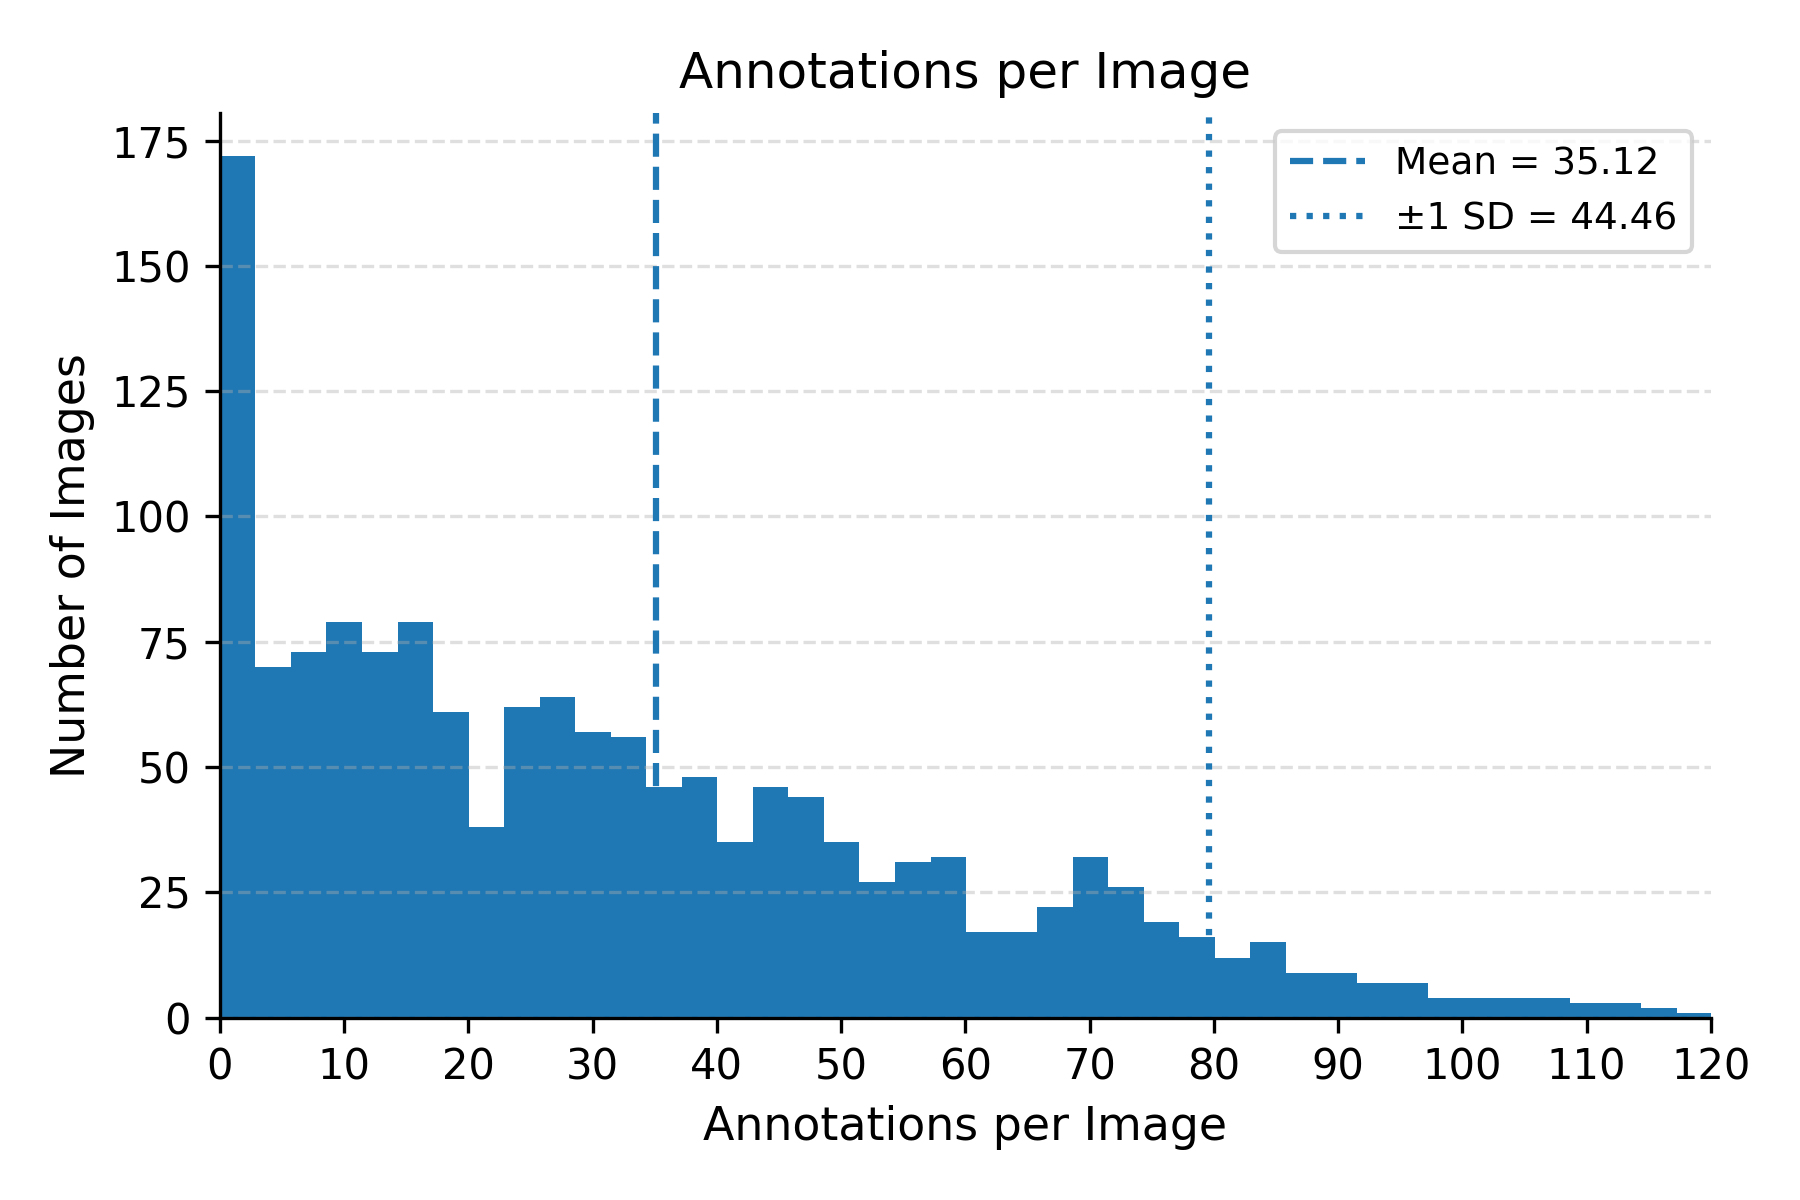
\includegraphics[width=0.75\linewidth]{images/Annotations per Image.png}
    \caption{Distribution of per–image annotation counts across the labeled dataset used to train the detectors. With a mean of 32 annotations per image with a wide standard deviation.}

    \label{fig:Annotations per Image}
\end{figure}

% -- Remove to simplify --
% Possibly due to the timing of the data collection, a majority of the blooms captured were of the late bloom stage. The timing that a flower would stay at the early stage bloom appeared to last for less than 24 hours, resulting in only a small amount of flowers actually being captured in this stage. After these flowers were open, they would remain intact on the uprights through multiple imaging sessions.

Due to the low number of early bloom flowers noted, they were merged into the larger group of total flower count that included all bloomed flowers regardless of stage.

\begin{equation}
\label{eq:TFC}
\text{Total Flower Count} = {\text{EB + LB}}
\end{equation}
\vspace{10pt}

An example of an annotated image with both Early and Late Blooms can be seen in Figure~\ref{fig:early and late bloom}

\begin{figure}[H]
    \centering
    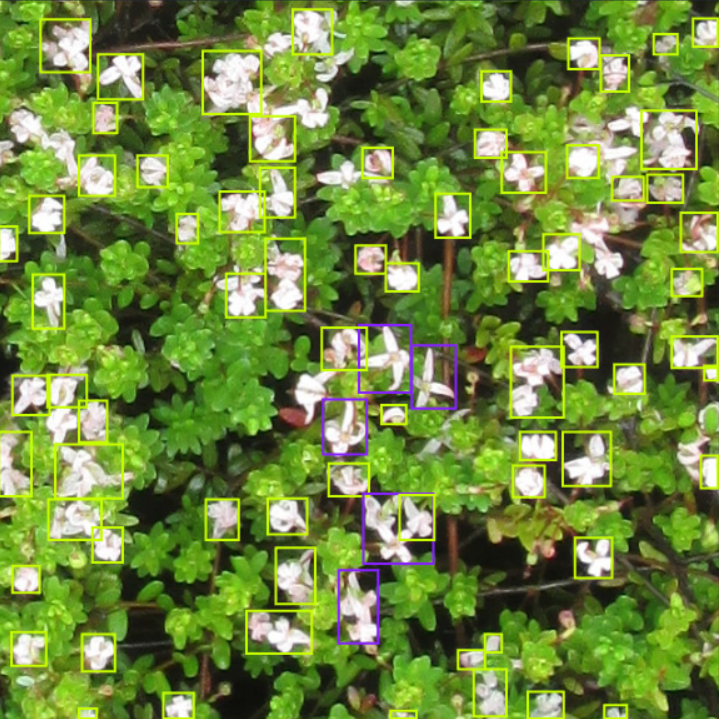
\includegraphics[width=0.5\linewidth]{images/Early and Late Bloom.png}
    \caption{Example annotated frame showing both Early Bloom (EB) and Late Bloom (LB) classes. Colored boxes indicate model targets; EB+LB defines the Total Flower Count used throughout the analysis. This illustration clarifies stage definitions and shows typical occlusion/lighting conditions encountered in the field.}
    \label{fig:early and late bloom}
\end{figure}

Both YOLO models and RF3 were trained to 150 epochs and the RF-DETR model was trained to 25 epochs. These training times are in line with current results as YOLO models often benefit from longer schedules due to heavy stochastic augmentation where longer schedules yield new views of the data and steady AP gains \cite{bochkovskiy_yolov4_2020}. In contrast, modern DETR-style models that RF-DETR builds on adopt architectural and training tweaks that accelerate convergence compared with the original DETR \cite{zhu_deformable_2021}. However, the original DETR needed ~500 epochs on COCO, whereas DINO reports competitive accuracy in just 12–24 epochs \cite{wang_rt-detrv3_2025}.

After training, the performance of each model is shown below in Table~\ref{tab:model-performance-comparison}. On the held-out test set, RF-DETR achieved the most accurate results with mAP@0.50 = 74.2\%, Precision = 77.0\%, Recall = 70.2\%; YOLOv12 performed the highest among the YOLO family of models tested and achieved mAP@0.50 = 69.3\%, Precision = 79.0\%, Recall = 66.4\%. The results for the time to inference test are also shown in Table~\ref{tab:inference time}. The inference time between v11, v12, and RF3 was very close, with v11 being slightly quicker as expected, and RF-DETR had significantly higher latency \cite{gonzalez_hernandez_analysis_2025}\cite{saltik_comparative_2025}.  

\begin{table}[!ht]
\centering
\caption{Model Performance Comparison}
\label{tab:model-performance-comparison}
\footnotesize
\setlength{\tabcolsep}{6pt}
\begin{tabular}{ccccc}
\toprule
\textbf{Model} & \textbf{mAP@50 (\%)} & \textbf{Precision (\%)} & \textbf{Recall (\%)} & \textbf{F1-Score (\%)} \\
\midrule
YOLOv11  & 67.1 & 68.7 & 71.6 & 70.1 \\
YOLOv12  & 69.3 & 79.0 & 66.4 & 71.9 \\
RF3      & 65.9 & 76.7 & 65.8 & 70.6 \\
RF-DETR  & 74.2 & 77.0 & 70.2 & 73.2 \\
\bottomrule
\end{tabular}
\end{table}

Comparing the models directly, RF-DETR favors global reasoning and end-to-end simplicity, YOLOv12 injects stronger attention for context while aiming to stay real-time, YOLOv11 maximizes efficiency within the classic convolutional recipe, and Roboflow 3 emphasizes ease of deployment. Based on this, we can select based on priority of accuracy/segmentation (RF-DETR), attention-driven context at speed (v12), edge-friendly throughput (v11), or smooth training-to-deployment workflows with flexible latency/accuracy trade-offs (RF3).


 We measured CPU inference latency on a Dell Precision 5550 (Intel i7-10850H, 64 GB RAM) with batch size = 1, input = 640$\times$640, 5 warm-up runs, and 25 timed runs per model, reporting average/median/P95 per-image latency in Table~\ref{tab:inference time}.

\begin{table}[!ht]
\centering
\caption{CPU Inference Time Summary}
\label{tab:inference time}
\footnotesize
\setlength{\tabcolsep}{6pt}
\begin{tabular}{ccccc}
\toprule
\textbf{Model} & \textbf{Timed Runs (N)} & \textbf{Avg Latency (ms)} & \textbf{Median (ms)} & \textbf{P95 (ms)} \\
\midrule
YOLOv12 & 25 & 205.98 & 212.60 & 223.72 \\
YOLOv11 & 25 & 184.17 & 183.88 & 205.26 \\
RF3 & 25 & 196.07 & 195.73 & 211.46 \\
RF-DETR & 25 & 683.50 & 682.44 & 724.35 \\
\bottomrule
\end{tabular}
\end{table}


This performance is found to be in line with current findings comparing these models \cite{kumar_container_2025}. Considering that all the models tested are state-of-the-art models and are typically built upon previous versions, the similarity in results is expected. Similar to relevant studies that have seen improvement \cite{yang_gtdr-yolov12_2025}, we also saw increased performance of YOLOv12 over YOLOv11. Recent work in blueberry breeding has demonstrated the use of YOLOv11-based pipelines to classify fruit maturity and provide a proxy for yield estimation, highlighting the potential of object detection frameworks for small fruit crops \cite{zhang_open-source_2024,li_high-throughput_2025}.

After the successful creation of the ML model, we used the YOLOv12 model to analyze thirty plots for yield correlation. Although RF-DETR achieved the highest mAP@0.50 (74.2\%), YOLOv12’s mAP was within 4.9 points, and the median CPU latency was 3.2$\times$ lower than RF-DETR at 640×640 (213 ms vs 682 ms). Due to the significant difference in inference time compared to mAP, we employed YOLOv12 for downstream plot analysis.  Plots were split into two groups based on genetic variation, one set of Stevens cultivar representing a control group and one set of Experimental variations with differing genetic traits. Plots were sampled three times at 5-day intervals from the end of June to early July, representing peak flowering timing. Using these images, we detected multiple stages of flower development and recorded flower counts per plot over the three imaging sessions. Using this new dataset, we compared the temporal flowering patterns of the two groups. The data collected is shown in Table~\ref{tab: Flower Count Data}. Plotting this data by group, we see a trend of decreasing flower count by date. It is also notable that the Stevens cultivar has less variability in flower count over time. 

%==================== Table B: Flower Counts ====================
\begin{table}[!ht]
\centering
\caption{Collected Data — Flower Counts}
\label{tab: Flower Count Data}
\footnotesize
\setlength{\tabcolsep}{4pt}
\adjustbox{max width=\textwidth}{%
\begin{tabular}{ccccc}
\toprule
\textbf{Plot Number} & \textbf{Type} & \textbf{22-June} & \textbf{27-June} & \textbf{2-July} \\
\midrule
1  & Experimental & 212 & 29  & 31  \\
2  & Experimental & 163 & 31  & 112 \\
3  & Stevens      & 186 & 104 & 43  \\
4  & Stevens      & 181 & 174 & 34  \\
5  & Stevens      & 147 & 47  & 34  \\
6  & Experimental & 125 & 123 & 92  \\
7  & Stevens      & 248 & 105 & 44  \\
8  & Experimental & 118 & 52  & 51  \\
9  & Stevens      & 207 & 139 & 13  \\
10 & Stevens      & 172 & 100 & 47  \\
11 & Experimental & 165 & 120 & 78  \\
12 & Stevens      & 206 & 86  & 44  \\
13 & Experimental & 130 & 78  & 47  \\
14 & Experimental & 95  & 83  & 21  \\
15 & Experimental & 237 & 229 & 41  \\
16 & Stevens      & 184 & 38  & 24  \\
17 & Experimental & 143 & 172 & 60  \\
18 & Experimental & 256 & 101 & 117 \\
19 & Experimental & 135 & 98  & 74  \\
20 & Experimental & 98  & 36  & 50  \\
21 & Stevens      & 110 & 69  & 28  \\
22 & Experimental & 208 & 256 & 158 \\
23 & Experimental & 206 & 60  & 87  \\
24 & Experimental & 102 & 105 & 53  \\
25 & Experimental & 162 & 39  & 36  \\
26 & Experimental & 120 & 104 & 17  \\
27 & Experimental & 185 & 96  & 72  \\
28 & Experimental & 85  & 95  & 78  \\
29 & Stevens      & 106 & 51  & 26  \\
30 & Experimental & 100 & 102 & 67  \\
\midrule
\textbf{Experimental Mean} &  & \textbf{152} & \textbf{100} & \textbf{67} \\
\textbf{Experimental Std}  &  & \textbf{51}  & \textbf{60}  & \textbf{35} \\
\textbf{Stevens Mean}      &  & \textbf{175} & \textbf{91}  & \textbf{34} \\
\textbf{Stevens Std}       &  & \textbf{44}  & \textbf{43}  & \textbf{11} \\
\bottomrule
\end{tabular}}
\end{table}


\begin{figure}[H]
    \centering
    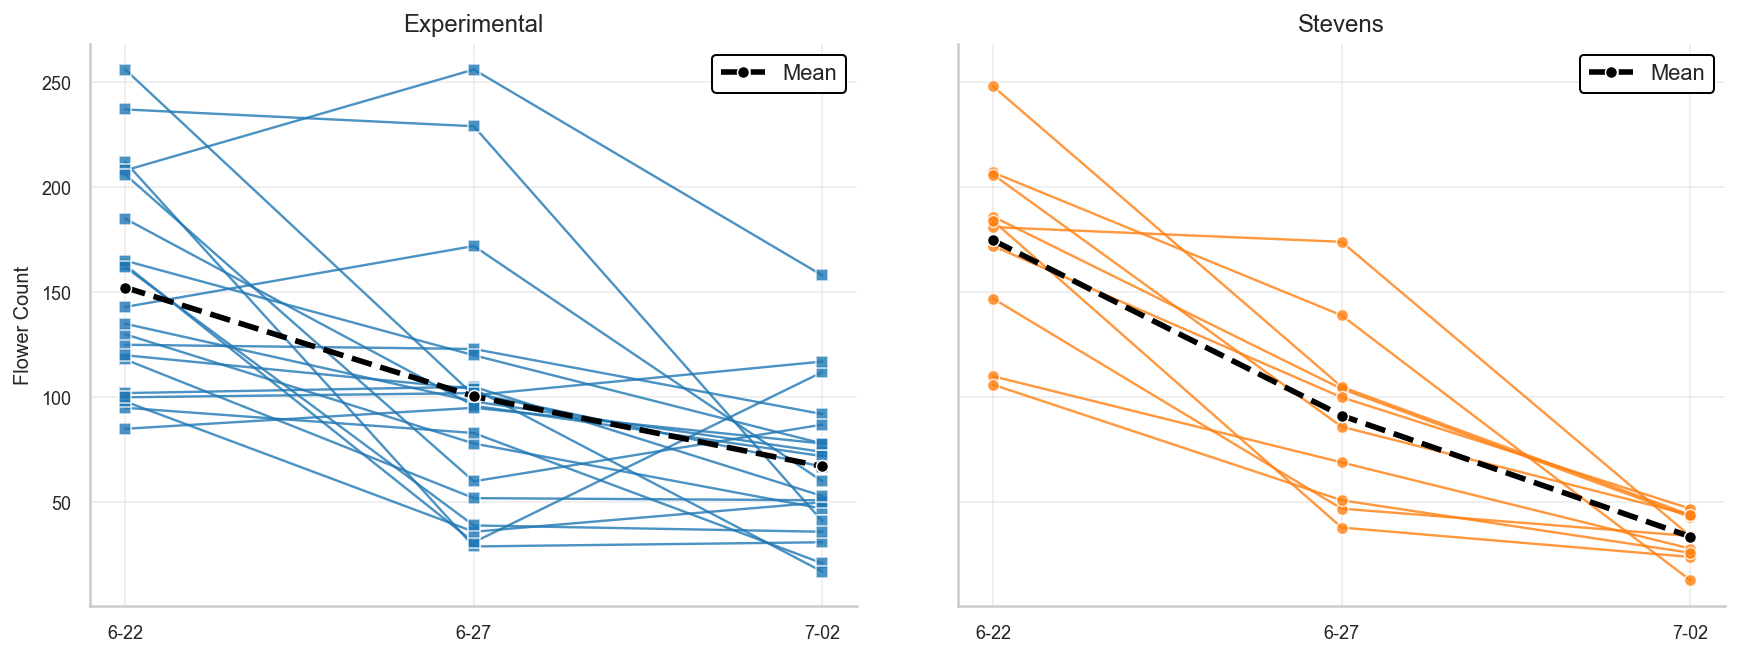
\includegraphics[width=0.85\linewidth]{images/Count by Type vs Date.png}
    \caption{Flower count by date, stratified by cultivar type (Stevens vs Experimental). Points are plot-level observations across three imaging sessions; the line traces the date-wise mean, highlighting bloom rise and peak timing by cohort. This view supports later yield analyses by establishing the temporal context of flowering intensity.}
    \label{fig:Count by Type vs Date}
\end{figure}

At the completion of the growing season, plots were sampled in the standard method of collecting all berries in a 300~mm~$\times$~300~mm quadrat on two separate days to generate a ground truth dataset. This data was recorded as fruit count and yield. This data is shown in Table~\ref{tab: Harvest Data}

%==================== Table A: Harvest 1 & Harvest 2 ====================
\begin{table}[!ht]
\centering
\caption{Collected Data — Harvest 1 and Harvest 2}
\label{tab: Harvest Data}
\footnotesize
\setlength{\tabcolsep}{4pt}
\adjustbox{max width=\textwidth}{%
\begin{tabular}{|c|c|c|c|c|c|c|c|c|c|}
\cline{3-10}
\multicolumn{1}{c}{} & \multicolumn{1}{c}{} & \multicolumn{4}{|c|}{Harvest 1} & \multicolumn{4}{c|}{Harvest 2} \\
\hline{}
\multirow{2}{*}{Plot Number} & \multirow{2}{*}{Type} & Good Count & Rotten Count & Good Yield & Rotten Yield & Good Count & Rotten Count & Good Yield & Rotten Yield \\
 &  & \textit{(Number of Berries)} & \textit{(Number of Berries)} & \textit{(g)} & \textit{(g)} & \textit{(Number of Berries)} & \textit{(Number of Berries)} & \textit{(g)} & \textit{(g)} \\
\hline
1 & Experimental & 232 & 32 & 315.1 & 41.4 & 131 & 15 & 199.7 & 15.6 \\
2 & Experimental & 125 & 63 & 172.0 & 63.0 & 54 & 36 & 81.6 & 47.3 \\
3 & Stevens      & 70  & 28 & 138.4 & 41.9 & 30  & 23 & 66.2 & 35.6 \\
4 & Stevens      & 49  & 19 & 80.5  & 22.3 & 39  & 47 & 84.4 & 78.2 \\
5 & Stevens      & 134 & 9  & 293.5 & 15.4 & 99  & 28 & 217.6 & 49.0 \\
6 & Experimental & 126 & 47 & 148.3 & 48.7 & 72  & 33 & 84.9 & 34.9 \\
7 & Stevens      & 60  & 38 & 117.8 & 62.8 & 89  & 138 & 186.7 & 228.5 \\
8 & Experimental & 90  & 48 & 116.4 & 50.9 & 95  & 120 & 145.6 & 143.7 \\
9 & Stevens      & 79  & 32 & 171.3 & 49.5 & 89  & 91 & 199.7 & 151.8 \\
10 & Stevens     & 139 & 38 & 258.0 & 67.3 & 67  & 26 & 145.8 & 40.0 \\
11 & Experimental & 143 & 35 & 219.6 & 40.9 & 33  & 57 & 59.9 & 81.8 \\
12 & Stevens     & 111 & 51 & 197.8 & 77.6 & 59  & 59 & 110.2 & 99.4 \\
13 & Experimental & 137 & 18 & 179.6 & 22.5 & 50  & 79 & 80.0 & 92.4 \\
14 & Experimental & 134 & 24 & 181.8 & 25.5 & 60  & 28 & 105.1 & 36.0 \\
15 & Experimental & 276 & 52 & 188.5 & 29.3 & 174 & 44 & 142.3 & 30.2 \\
16 & Stevens     & 78  & 13 & 140.5 & 17.3 & 31  & 7  & 62.3 & 12.5 \\
17 & Experimental & 108 & 121 & 108.6 & 106.3 & 39 & 94 & 41.9 & 99.4 \\
18 & Experimental & 97  & 84 & 121.2 & 92.6 & 59  & 98 & 84.7 & 111.6 \\
19 & Experimental & 129 & 5  & 153.5 & 4.3 & 132 & 11 & 176.0 & 14.1 \\
20 & Experimental & 148 & 20 & 174.8 & 21.2 & 92  & 94 & 140.8 & 112.3 \\
21 & Stevens     & 55  & 3  & 127.9 & 2.9 & 70  & 24 & 157.4 & 52.9 \\
22 & Experimental & 297 & 3  & 170.0 & 1.7 & 246 & 16 & 155.3 & 9.7 \\
23 & Experimental & 127 & 19 & 162.0 & 19.4 & 124 & 50 & 155.2 & 61.2 \\
24 & Experimental & 120 & 15 & 152.7 & 15.0 & 94  & 85 & 137.7 & 101.1 \\
25 & Experimental & 113 & 94 & 137.5 & 75.2 & 102 & 64 & 138.6 & 69.6 \\
26 & Experimental & 82  & 62 & 97.9  & 61.0 & 42  & 62 & 55.7 & 74.9 \\
27 & Experimental & 207 & 22 & 164.4 & 15.8 & 190 & 47 & 143.3 & 35.3 \\
28 & Experimental & 86  & 66 & 114.8 & 70.9 & 36  & 142 & 53.6 & 166.5 \\
29 & Stevens     & 99  & 15 & 211.9 & 19.7 & 89  & 35 & 186.6 & 59.2 \\
30 & Experimental & 140 & 27 & 169.6 & 27.0 & 64  & 36 & 86.7 & 34.2 \\
\hline
\rowcolor{lightgray} Experimental Mean &  & \textbf{146} & \textbf{43} & \textbf{162.4} & \textbf{41.6} & \textbf{94} & \textbf{42} & \textbf{113.4} & \textbf{68.6} \\
\rowcolor{lightgray} Experimental Std  &  & \textbf{60}  & \textbf{31} & \textbf{47.3}  & \textbf{29.0} & \textbf{57} & \textbf{29} & \textbf{45.3}  & \textbf{44.4} \\
\rowcolor{lightgray} Stevens Mean      &  & \textbf{87}  & \textbf{25} & \textbf{173.8} & \textbf{37.7} & \textbf{66} & \textbf{38} & \textbf{141.7} & \textbf{80.7} \\
\rowcolor{lightgray} Stevens Std       &  & \textbf{32}  & \textbf{15} & \textbf{66.5}  & \textbf{25.7} & \textbf{26} & \textbf{26} & \textbf{57.5}  & \textbf{64.8} \\
\hline
\end{tabular}}
\end{table}


Due to a relatively low sample size of both Stevens and Experimental plots, 10 plots and 20 plots respectively, it was decided to also consider the total berry count of both harvests and total flower count from all sessions as an additional dataset. 

\begin{figure}[!ht]
  \begin{subfigure}{0.45\textwidth}
    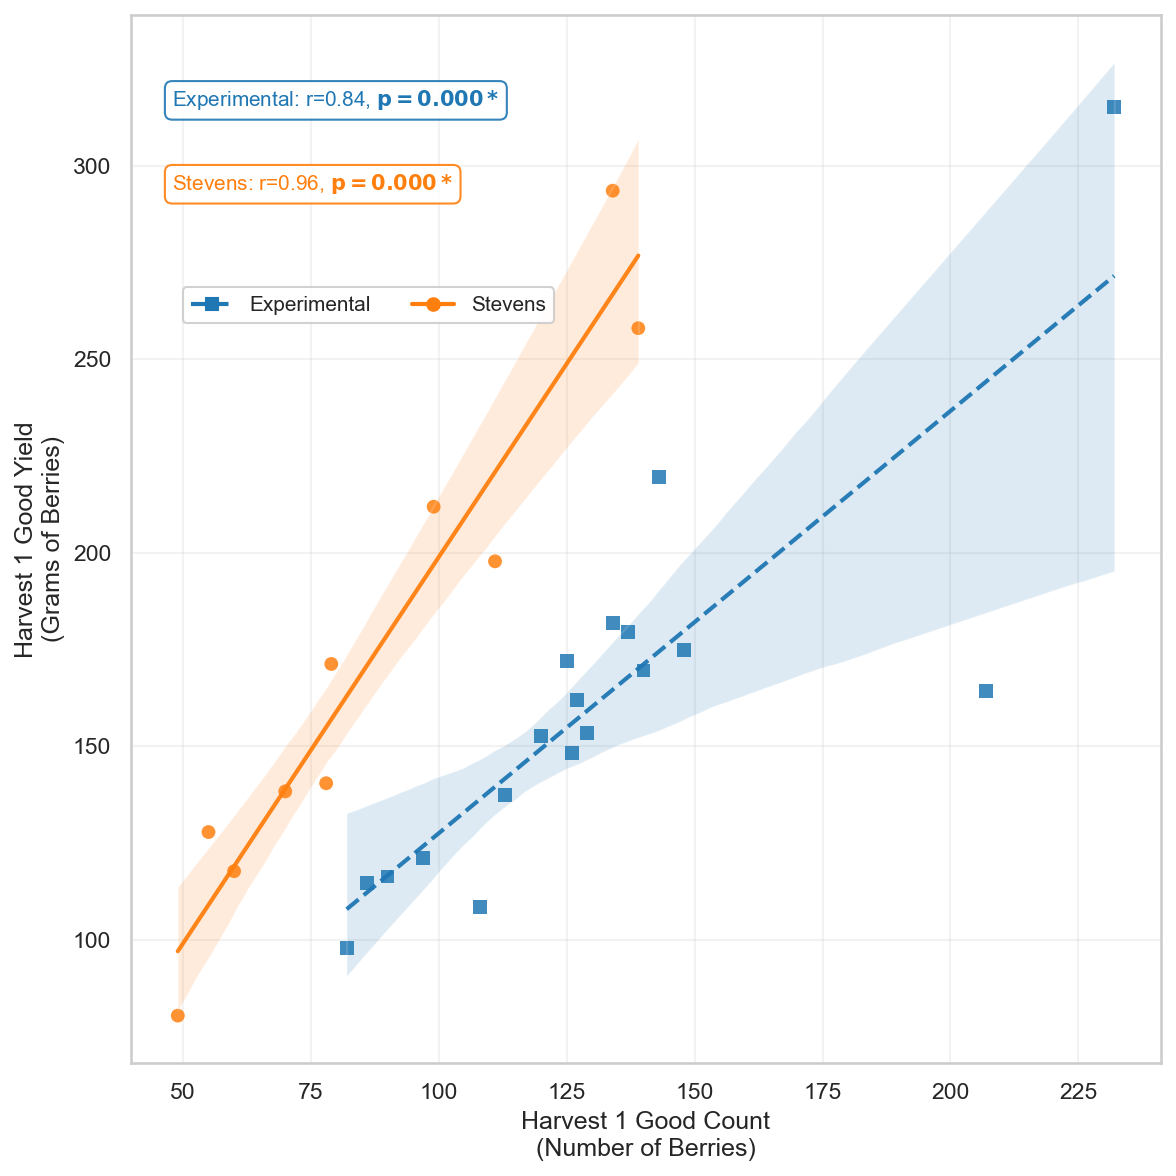
\includegraphics[width=\textwidth]{images/h1-countvsyield.png}
   \caption{Harvest 1 Count vs Yield}
    \label{fig:H1 Count vs Yield}
  \end{subfigure}
  \hfill
  \begin{subfigure}{0.45\textwidth}
    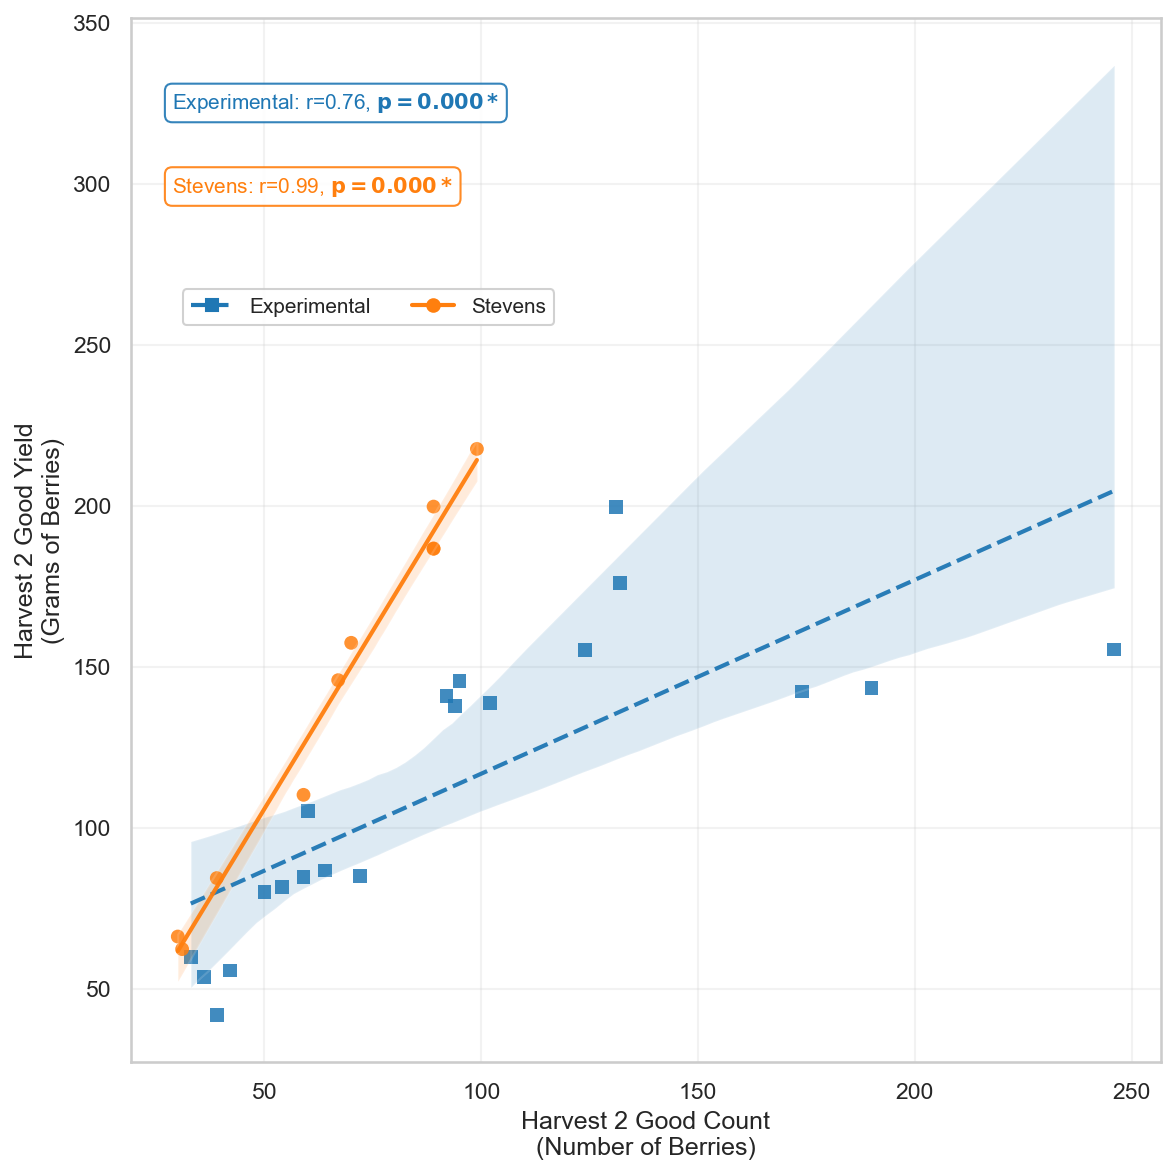
\includegraphics[width=\textwidth]{images/h2-countvsyield.png}
   \caption{Harvest 2 Count vs Yield}
    \label{fig:H2 count to yield}
  \end{subfigure}
  \caption{Relationship between plot-level berry count and measured yield for (a) Harvest 1 and (b) Harvest 2. Lines show ordinary least squares (OLS) fits; shaded bands are 95\% confidence intervals. Strong positive associations across both harvests justify using berry counts as a proxy for yield and provide a baseline for linking early flowering to end-of-season outcomes.}
  \label{fig:Harvest count comparison}
\end{figure}

 Pearson’s r (two-tailed p) was computed with SciPy \cite{virtanen_scipy_2020} and visualized with seaborn.\cite{waskom_seaborn_2021} The Pearson’s correlation coefficient (r) quantifies the strength and direction of the linear association between two continuous variables by standardizing their covariance. We used Pearson's r with two-tailed p-values to summarize pairwise relationships, noting it captures linear dependence\cite{sedgwick_pearsons_2012}.

 In order to ensure a robust relationship between flower count and yield, the correlation between harvest counts and yield was first needed. Figure~\ref{fig:Harvest count comparison} shows a strong correlation between berry count and yield of the Experimental cultivar in both Harvest 1 and Harvest 2, \rnp{0.76}{20}{<.001} and \rnp{0.84}{20}{<.001} respectively. This trend was also seen in the Stevens cultivar, with the correlation between berry count and yield in Harvest 1 and Harvest 2 being \rnp{0.96}{10}{<.001} and \rnp{0.99}{10}{<.001}. This mirrors work in blueberries demonstrating that berry number is the primary driver of yield and can serve as a reliable predictor \cite{salvo_estimate_2012,percival_narrow_2012}. Additionally, this correlation shows a consistency of berry mass and distinctly a greater consistency in the Stevens plots, which is expected as these plots have reduced genetic diversity and more consistent fruit sizing \cite{gallardo_breeding_2018}.


Next, the correlation between flower count and berry count was investigated. Due to the high number of datasets consisting of three flowering dates, a total flower count, in addition to two harvest dates and their totals, a pair plot was used to find relevant correlation, as shown in Figure~\ref{fig:Flower Pair-Plot} found in the Appendix. 


\begin{figure}[!ht]
  \begin{subfigure}{0.45\textwidth}
    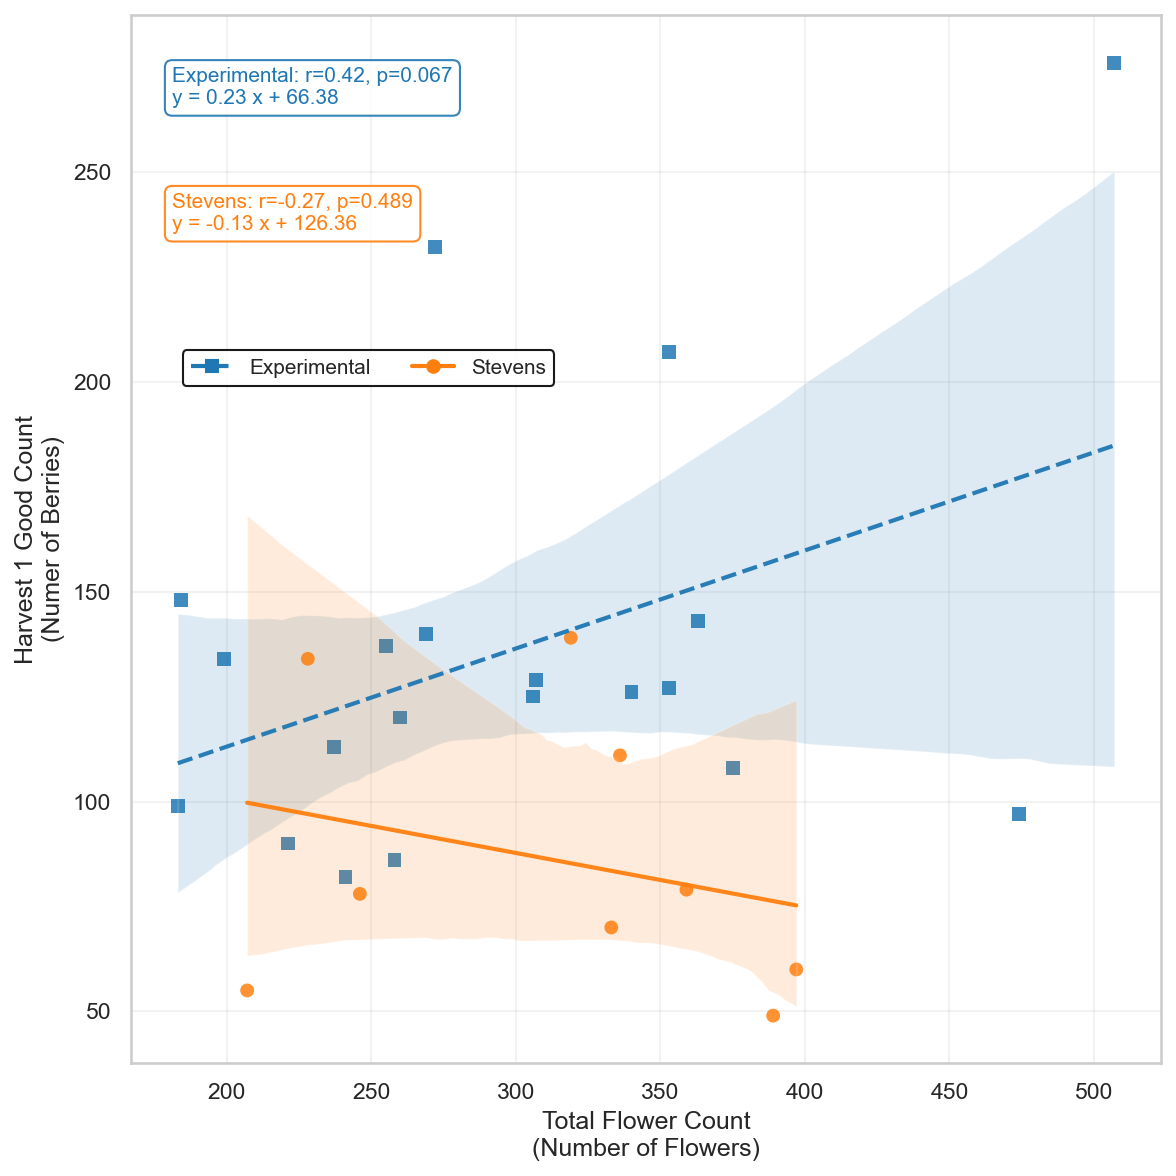
\includegraphics[width=\textwidth]{images/H1 GC vs TFC.png}
   \caption{Harvest 1 Good Count vs Total Flower Count}
    \label{fig:H1 GC vs TFC}
  \end{subfigure}
  \hfill
  \begin{subfigure}{0.45\textwidth}
    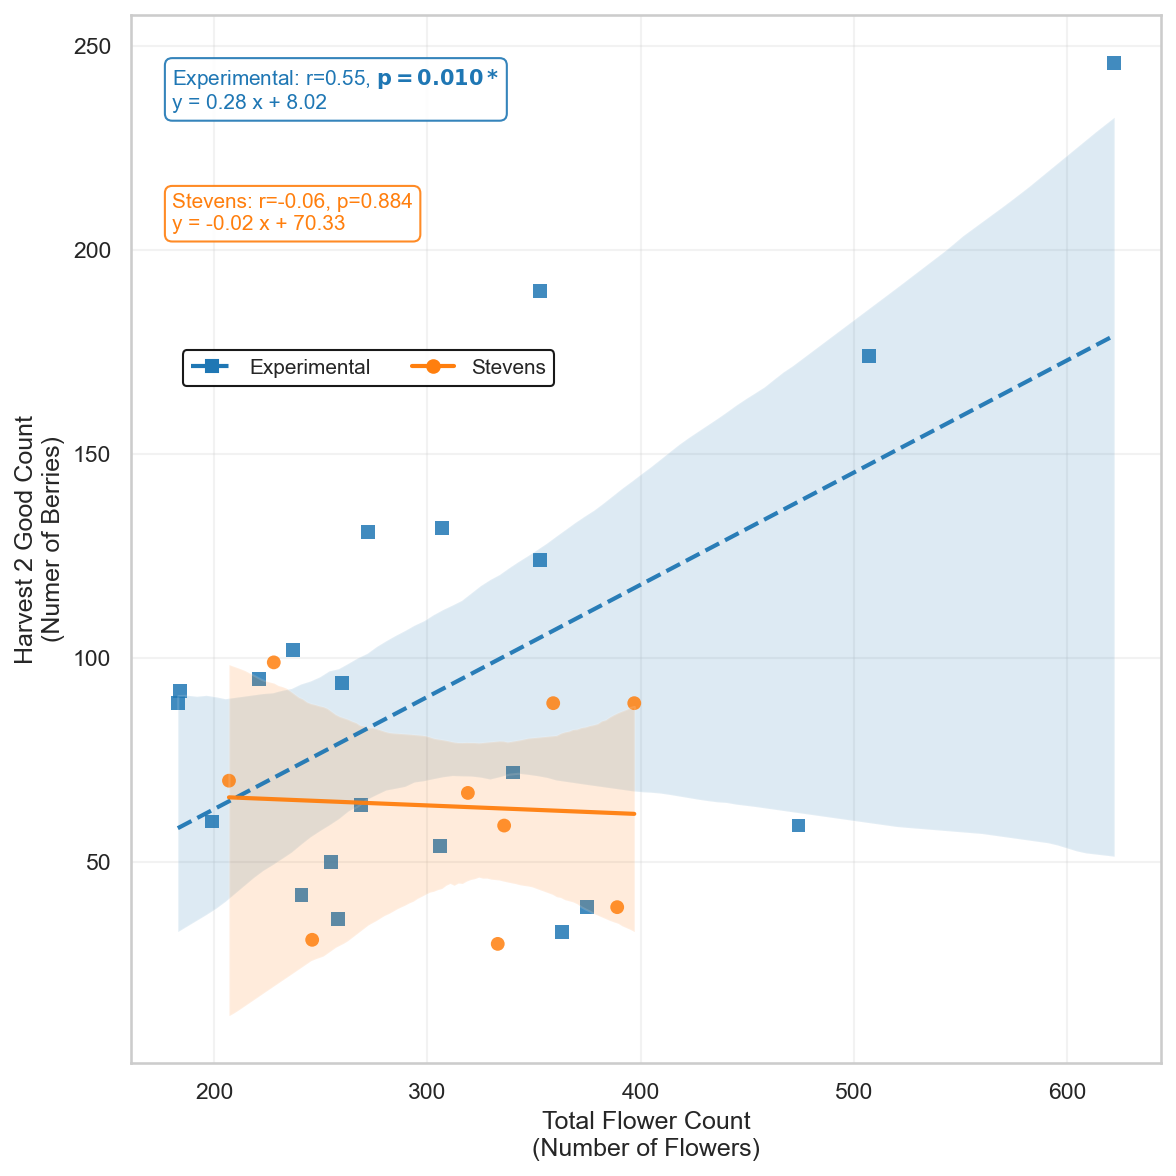
\includegraphics[width=\textwidth]{images/H2 GC vs TFC.png}
   \caption{Harvest 2 Good Count vs Total Flower Count}
    \label{fig:H2 GC vs TFC}
  \end{subfigure}
  \caption{Good berry count at (a) Harvest 1 and (b) Harvest 2 versus Total Flower Count (sum of Early + Late blooms). Points are plot-level values by cultivar; OLS lines with 95\% confidence bands summarize the trend. Experimental hybrids show a moderate to significant association, while Stevens differs, motivating cultivar-specific interpretation of flower-to-fruit conversion and possible variation in ripening dynamics.}
  \label{fig:GC vs TFC}
\end{figure}


When comparing flower counts to good berry count, however, results were more nuanced as seen in Figure~\ref{fig:GC vs TFC}. Experimental hybrids showed a moderate but significant correlation between total flower count and good berry count \rnp{0.55}{20}{= .010}. Stevens, in contrast, exhibited stronger correlations between total flower count and rotten berry count \rnp{0.70}{10}{= .034} as seen in Figure~\ref{fig:RC vs TFC}. This divergence may reflect cultivar-specific ripening dynamics, with Stevens plots appearing to have fruit overripen before harvest, resulting in higher rot incidence, while Experimental hybrids were closer to peak ripening at the time of collection. Some cultivar-dependent differences in flower-to-fruit conversion efficiency and fruit quality outcomes have been documented in blueberry production \cite{cortes-rivas_pollination_2023} and differences in fruit quality outcomes—such as berry size, mass, color, and biochemistry—have been well documented in cranberry breeding populations \cite{loarca_berryportraits_2024,maule_buds_2024}.

\begin{figure}[!ht]
  \begin{subfigure}{0.5\textwidth}
    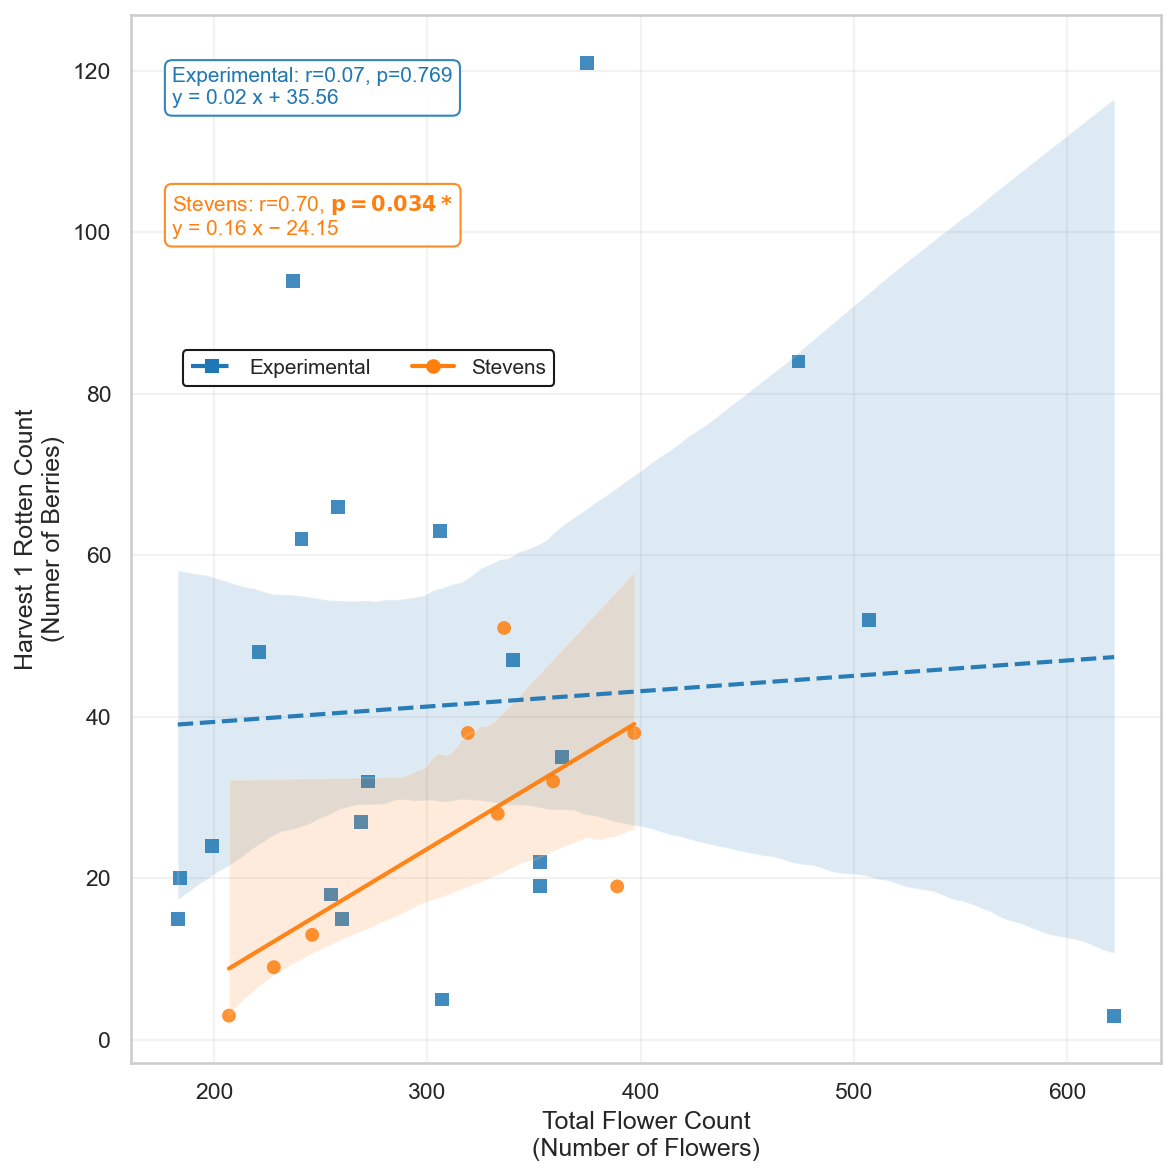
\includegraphics[width=\textwidth]{images/H1 RC vs TFC.png}
   \caption{Harvest 1 Rotten Count vs Total Flower Count}
    \label{fig:H1 RC vs TFC}
  \end{subfigure}
  \hfill
  \begin{subfigure}{0.5\textwidth}
    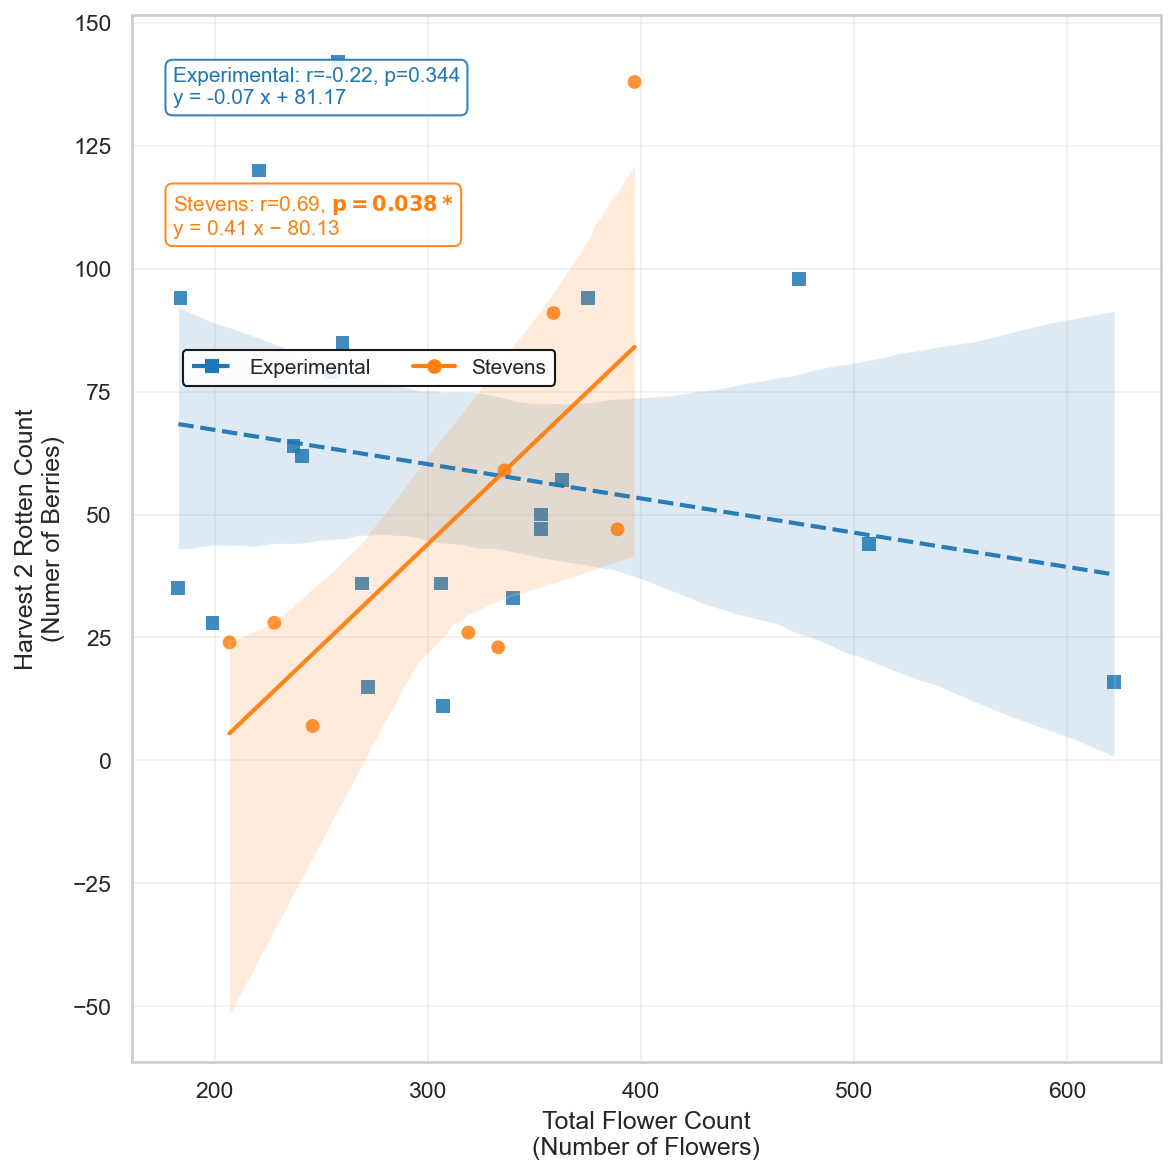
\includegraphics[width=\textwidth]{images/H2 RC vs TFC.png}
   \caption{Harvest 2 Rotten Count vs Total Flower Count}
    \label{fig:H2 RC vs TFC}
  \end{subfigure}
  \caption{Rotten berry count at (a) Harvest 1 and (b) Harvest 2 versus Total Flower Count. OLS fits with 95\% CIs reveal a stronger positive association for Stevens than for Experimental hybrids, likely due to cultivar-dependent ripening dynamics and post-set losses that raise rot incidence in Stevens under the season’s conditions.}
  \label{fig:RC vs TFC}
\end{figure}

In Figure~\ref{fig:TBC vs TFC}, total flower count is positively associated with total berry count. The relationship is moderate and statistically significant in the Experimental hybrids \rnp{0.68}{20}{= .001}, but weaker and not significant in Stevens \rnp{0.39}{10}{= .304}. This divergence is consistent with cultivar-specific dynamics noted earlier (e.g., greater post-set losses/rot in Stevens), indicating that flower abundance provides a more reliable early yield signal in the Experimental cohort under this season’s conditions. Practically, plots with more flowers tended to produce more berries, supporting flower counts as a viable, image-based proxy for eventual berry set.


\begin{figure}[H]
    \centering
    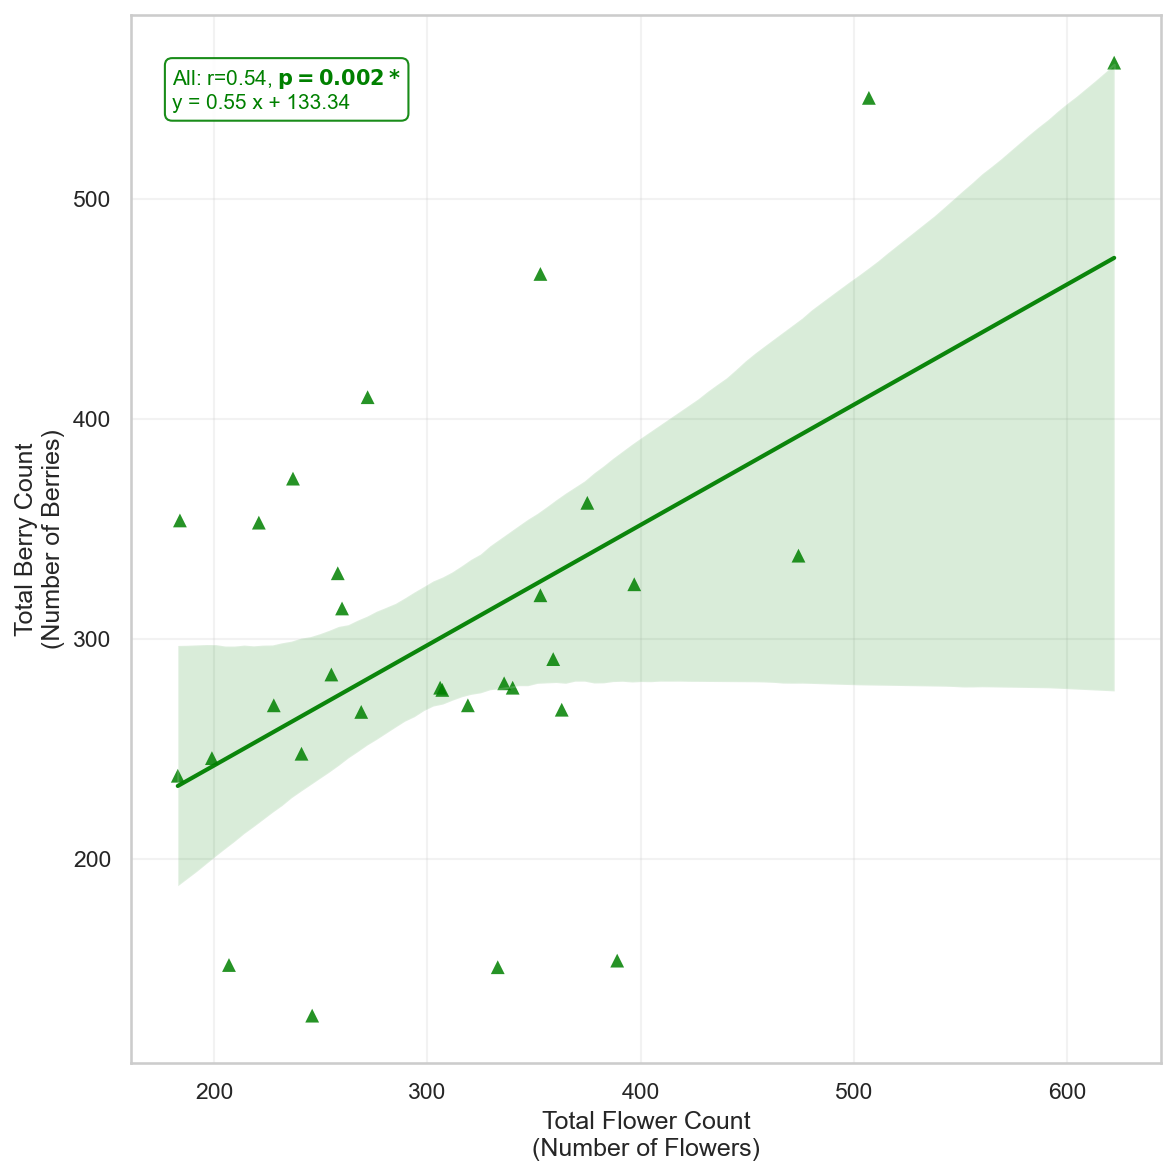
\includegraphics[width=0.75\linewidth]{images/TBC to TFC all Cultivars.png}
    \caption{Total Berry Count (both harvests combined) versus Total Flower Count aggregated over the standardized bloom window. Each point is a plot; the OLS fit with 95\% CI shows a clear, positive relationship overall and a stronger signal in the Experimental cultivars. This supports using early flower abundance as an image-based indicator of expected berry number under similar conditions.}
    \label{fig:TBC vs TFC APT}
\end{figure}

\begin{figure}[H]
    \centering
    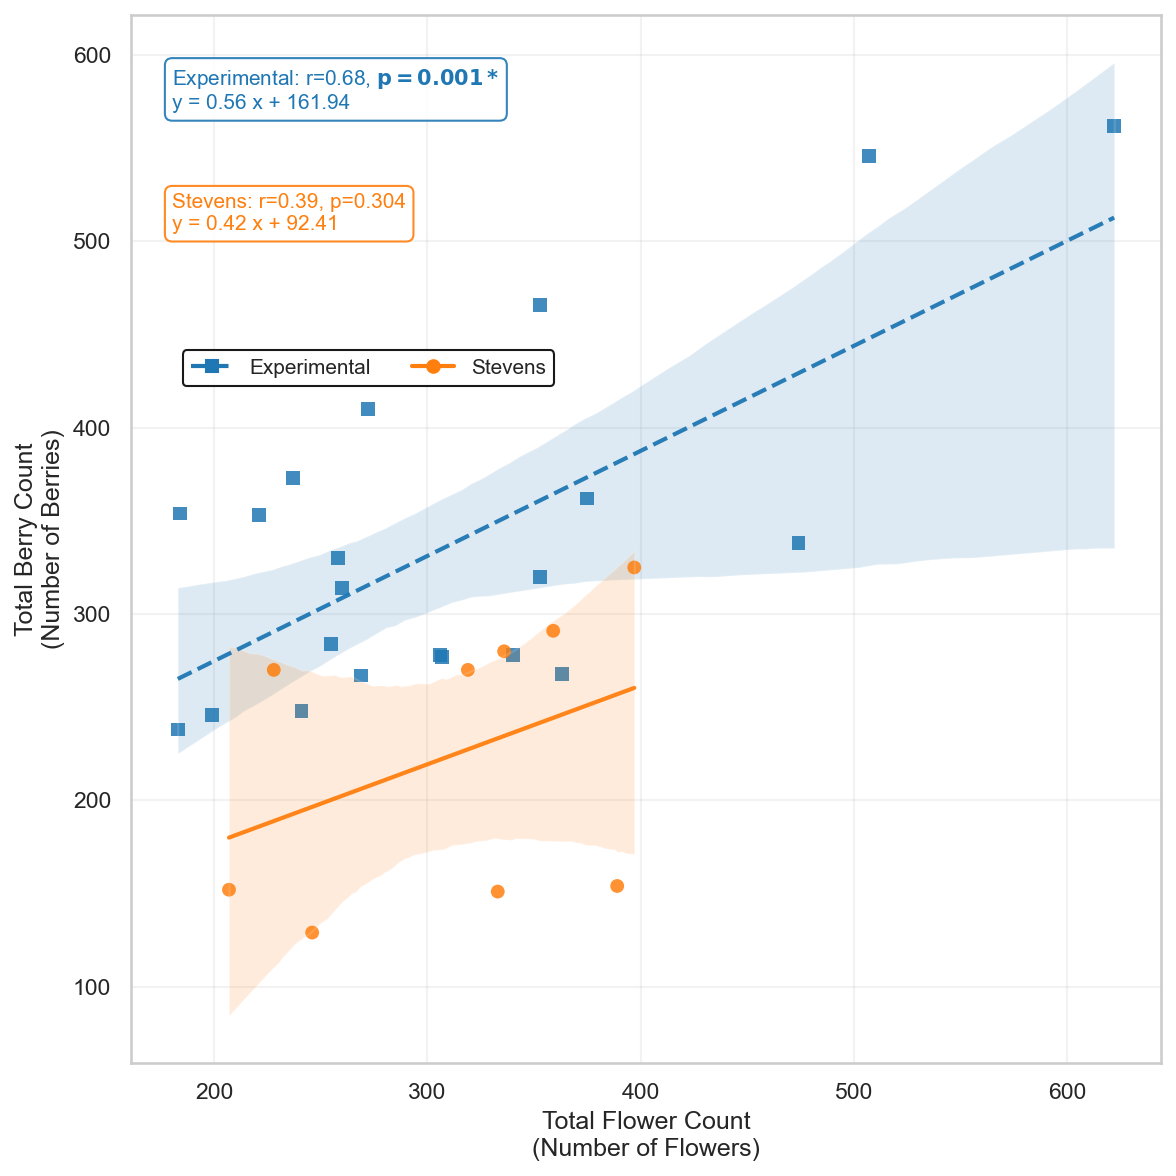
\includegraphics[width=0.75\linewidth]{images/TBC vs TFC.png}
    \caption{Total Berry Count across all harvests and cultivars versus Total Flower Count over the bloom window with no distinction between cultivar types. the OLS fit with 95\% CI shows a clear, positive relationship overall and a strong correlation. This supports using early flower abundance as an image-based indicator of expected berry number under similar conditions.}
    \label{fig:TBC vs TFC}
\end{figure}


\section{Conclusion}
We demonstrated an end-to-end workflow from ground image capture, assisted annotation, and object-detection modeling—that is then able to detect and count cranberry flowers to be used to predict berry count. Among four modern detectors, YOLOv12 offered the best accuracy/latency trade-off for edge deployment (mAP@0.50 = 69.3\%, F1 = 71.9\%), with inference latency $\approx$3.2$\times$ lower than RF-DETR at 640$\times$640. We then used the YOLOv11 model to quantify relationships between flowering and harvest outcomes across 30 plots. Total flower count moderately predicted total berry count in Experimental hybrids \rnp{0.68}{20}{= .001}, while cultivar-specific ripening patterns likely contributed to the stronger association between flowers and rot in Stevens. 

These findings suggest that low-cost cameras combined with on-device inference can provide growers with useful yield estimates several weeks before harvest. Compared with manual quadrat sampling, automated imaging increases spatial coverage and temporal frequency, improving robustness to within-bed variability. 

Future work should refine class definitions, establish standardized imaging schedules to distinguish pollination success from post-set fruit loss, and increase imaging frequency to improve predictive accuracy. A larger, multi-site study with standardized imaging windows and pre-specified analyses will help translate these early correlations into calibrated, cultivar-aware yield predictors suitable for commercial adoption.

\section{References}

\printbibliography[heading=none]


\appendix
\chapter*{Appendix A}
\addcontentsline{toc}{chapter}{Appendix A} % if you want it in the TOC

\begin{table}[!ht]
\centering
\caption{Full Collected Data}
\label{tab: full collected data}
\footnotesize
\setlength{\tabcolsep}{4pt}
\adjustbox{max width=\textwidth}{%
\begin{tabular}{|c|c|c|c|c|c|c|c|c|c|c|c|c|}
\hline
 & & \multicolumn{4}{c|}{Harvest 1} & \multicolumn{4}{c|}{Harvest 2} & \multicolumn{3}{c|}{Flower Counts} \\
\hline
Plot Number & Type & Good Count & Rotten Count & Good Yield & Rotten Yield & Good Count & Rotten Count & Good Yield & Rotten Yield & 22-June & 27-June & 02-July \\
\hline
1 & Experimental & 232 & 32 & 315.1 & 41.4 & 131 & 15 & 199.7 & 15.6 & 212 & 29 & 31 \\
2 & Experimental & 125 & 63 & 172.0 & 63.0 & 54 & 36 & 81.6 & 47.3 & 163 & 31 & 112 \\
3 & Stevens & 70 & 28 & 138.4 & 41.9 & 30 & 23 & 66.2 & 35.6 & 186 & 104 & 43 \\
4 & Stevens & 49 & 19 & 80.5 & 22.3 & 39 & 47 & 84.4 & 78.2 & 181 & 174 & 34 \\
5 & Stevens & 134 & 9 & 293.5 & 15.4 & 99 & 28 & 217.6 & 49.0 & 147 & 47 & 34 \\
6 & Experimental & 126 & 47 & 148.3 & 48.7 & 72 & 33 & 84.9 & 34.9 & 125 & 123 & 92 \\
7 & Stevens & 60 & 38 & 117.8 & 62.8 & 89 & 138 & 186.7 & 228.5 & 248 & 105 & 44 \\
8 & Experimental & 90 & 48 & 116.4 & 50.9 & 95 & 120 & 145.6 & 143.7 & 118 & 52 & 51 \\
9 & Stevens & 79 & 32 & 171.3 & 49.5 & 89 & 91 & 199.7 & 151.8 & 207 & 139 & 13 \\
10 & Stevens & 139 & 38 & 258.0 & 67.3 & 67 & 26 & 145.8 & 40.0 & 172 & 100 & 47 \\
11 & Experimental & 143 & 35 & 219.6 & 40.9 & 33 & 57 & 59.9 & 81.8 & 165 & 120 & 78 \\
12 & Stevens & 111 & 51 & 197.8 & 77.6 & 59 & 59 & 110.2 & 99.4 & 206 & 86 & 44 \\
13 & Experimental & 137 & 18 & 179.6 & 22.5 & 50 & 79 & 80.0 & 92.4 & 130 & 78 & 47 \\
14 & Experimental & 134 & 24 & 181.8 & 25.5 & 60 & 28 & 105.1 & 36.0 & 95 & 83 & 21 \\
15 & Experimental & 276 & 52 & 188.5 & 29.3 & 174 & 44 & 142.3 & 30.2 & 237 & 229 & 41 \\
16 & Stevens & 78 & 13 & 140.5 & 17.3 & 31 & 7 & 62.3 & 12.5 & 184 & 38 & 24 \\
17 & Experimental & 108 & 121 & 108.6 & 106.3 & 39 & 94 & 41.9 & 99.4 & 143 & 172 & 60 \\
18 & Experimental & 97 & 84 & 121.2 & 92.6 & 59 & 98 & 84.7 & 111.6 & 256 & 101 & 117 \\
19 & Experimental & 129 & 5 & 153.5 & 4.3 & 132 & 11 & 176.0 & 14.1 & 135 & 98 & 74 \\
20 & Experimental & 148 & 20 & 174.8 & 21.2 & 92 & 94 & 140.8 & 112.3 & 98 & 36 & 50 \\
21 & Stevens & 55 & 3 & 127.9 & 2.9 & 70 & 24 & 157.4 & 52.9 & 110 & 69 & 28 \\
22 & Experimental & 297 & 3 & 170.0 & 1.7 & 246 & 16 & 155.3 & 9.7 & 208 & 256 & 158 \\
23 & Experimental & 127 & 19 & 162.0 & 19.4 & 124 & 50 & 155.2 & 61.2 & 206 & 60 & 87 \\
24 & Experimental & 120 & 15 & 152.7 & 15.0 & 94 & 85 & 137.7 & 101.1 & 102 & 105 & 53 \\
25 & Experimental & 113 & 94 & 137.5 & 75.2 & 102 & 64 & 138.6 & 69.6 & 162 & 39 & 36 \\
26 & Experimental & 82 & 62 & 97.9 & 61.0 & 42 & 62 & 55.7 & 74.9 & 120 & 104 & 17 \\
27 & Experimental & 207 & 22 & 164.4 & 15.8 & 190 & 47 & 143.3 & 35.3 & 185 & 96 & 72 \\
28 & Experimental & 86 & 66 & 114.8 & 70.9 & 36 & 142 & 53.6 & 166.5 & 85 & 95 & 78 \\
29 & Stevens & 99 & 15 & 211.9 & 19.7 & 89 & 35 & 186.6 & 59.2 & 106 & 51 & 26 \\
30 & Experimental & 140 & 27 & 169.6 & 27.0 & 64 & 36 & 86.7 & 34.2 & 100 & 102 & 67 \\
\rowcolor{lightgray} Experimental Mean &  & \textbf{146} & \textbf{43} & \textbf{162.4} & \textbf{41.6} & \textbf{94} & \textbf{42} & \textbf{113.4} & \textbf{68.6} & \textbf{152} & \textbf{100} & \textbf{67} \\
\rowcolor{lightgray} Experimental Std &  & \textbf{60} & \textbf{31} & \textbf{47.3} & \textbf{29.0} & \textbf{57} & \textbf{29} & \textbf{45.3} & \textbf{44.4} & \textbf{51} & \textbf{60} & \textbf{35} \\
\rowcolor{lightgray} Stevens Mean &  & \textbf{87} & \textbf{25} & \textbf{173.8} & \textbf{37.7} & \textbf{66} & \textbf{38} & \textbf{141.7} & \textbf{80.7} & \textbf{175} & \textbf{91} & \textbf{34} \\
\rowcolor{lightgray} Stevens Std &  & \textbf{32} & \textbf{15} & \textbf{66.5} & \textbf{25.7} & \textbf{26} & \textbf{26} & \textbf{57.5} & \textbf{64.8} & \textbf{44} & \textbf{43} & \textbf{11} \\
\hline
\end{tabular}}
\end{table}


\newpage

\begin{figure}[H]
    \centering
    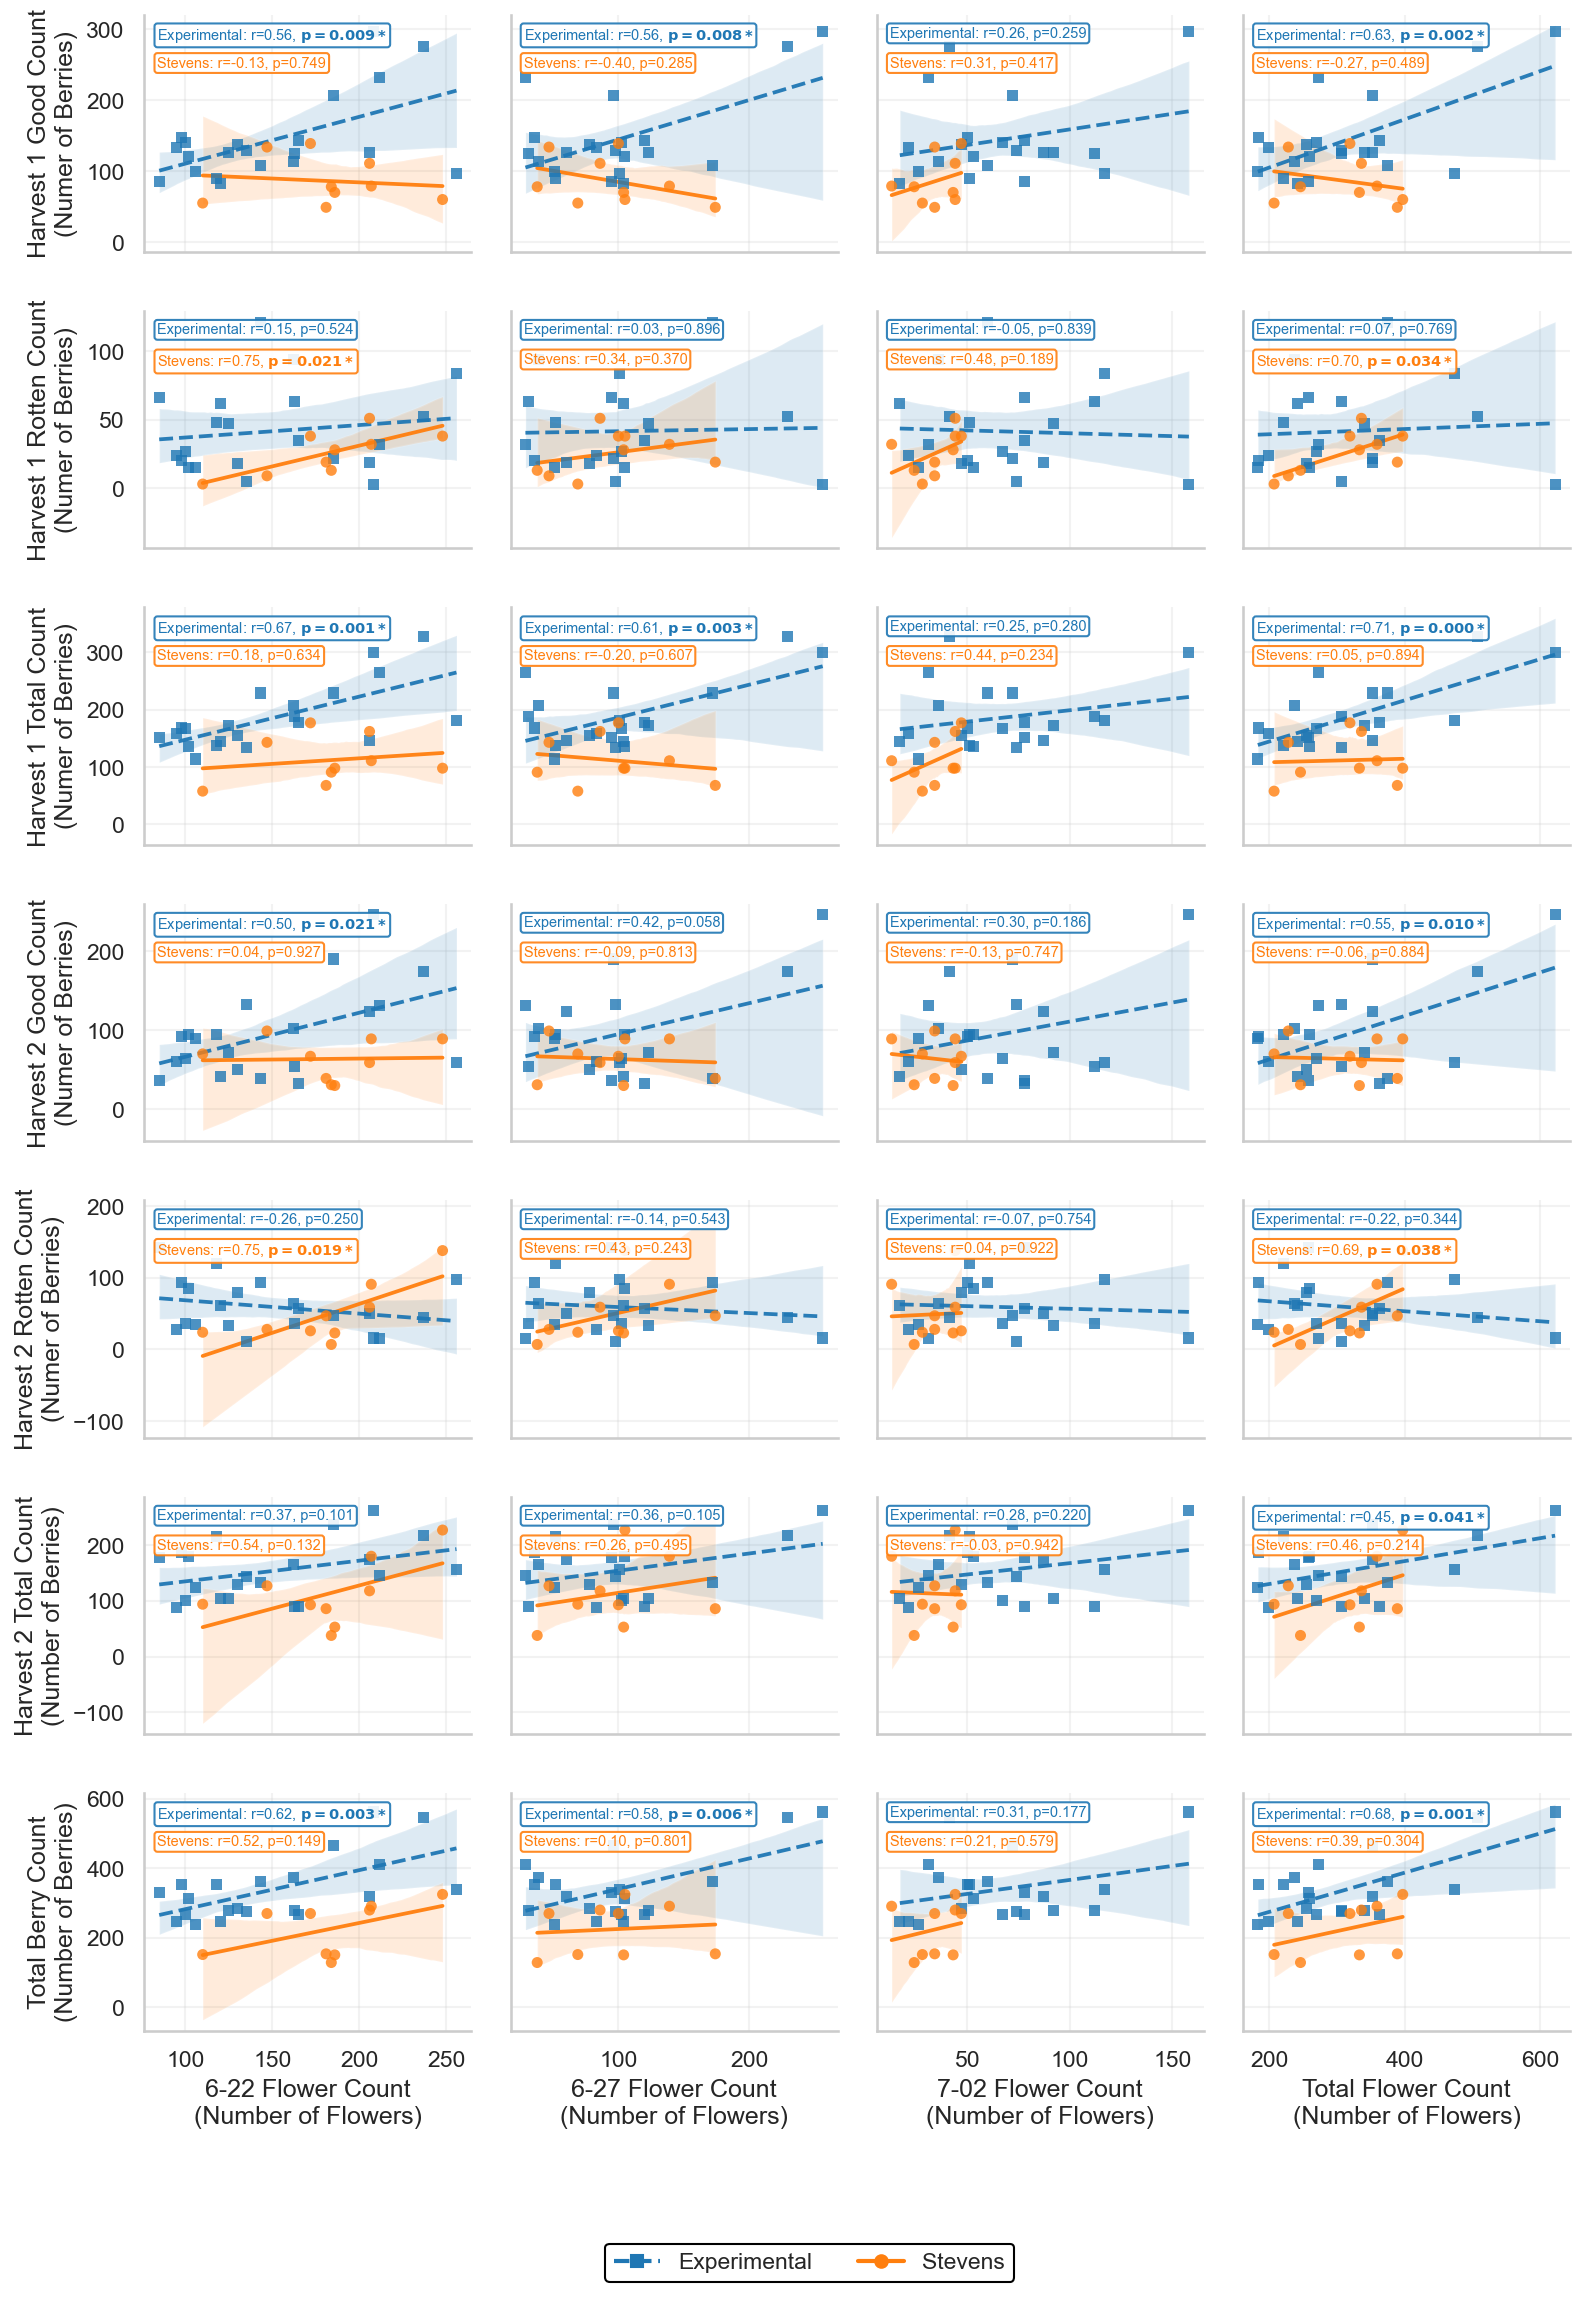
\includegraphics[width=1\linewidth]{images/Flower pair-plot.png}
    \caption{Pair-Plot of Berry Counts vs Flowering Counts}
    \label{fig:Flower Pair-Plot}
\end{figure}



\end{document}
